\documentclass[10pt, a4paper, twoside]{article}

% Mój kompilator tego nie obsłuży
% \usepackage{fontspec}
% \setmainfont{Arial}

\usepackage[utf8]{inputenc}
\usepackage[MeX]{polski}
\usepackage{graphicx}
\usepackage{amsmath,amssymb}
\usepackage{pdfpages} % paczka żeby móc importować gotowe strony z plików pdf do pdfa z latexa
\usepackage{titlesec} % może być potrzebne jeśli będziemy chcieli edytować tytuły

% First {} is a font size for title of sections and second {} is baselineskip,
% that is size of empty space between section title and text below
\titleformat{\section}
  {\normalfont\fontsize{12}{15}\bfseries}{\thesection}{1em}{\MakeUppercase}
\titleformat{\subsection}
  {\normalfont\fontsize{10}{12}\bfseries\itshape}{\thesubsection}{1em}{}
\titleformat{\subsubsection}
  {\normalfont\fontsize{10}{12}\itshape\selectfont}{\thesubsubsection}{1em}{}

% Uwaga, nie dodawać biblioteki sectsty bo to zresetuje formatowanie

\usepackage{tocloft}  % żeby móc ręcznie dodawać sections do TOC (Table of Content)
\usepackage[nottoc]{tocbibind}  % definiuje co jest w TOC
% nottoc -  Disables the inclusion of the ToC.

% to powyższe można zastąpić 2 liniami:
% \usepackage{tocbibind}
% \tocbibind{nottoc}

\usepackage{geometry} % Do ustawiania wyglądu stron
\geometry{margin=1.2in} % Ustawia margines

\usepackage{indentfirst}  % Ustawienia aby pierwszy paragraf w sekcji też miał akapit, bo domyślnie nie ma

\usepackage{graphicx} % Do załączania obrazów
\graphicspath{ {./images/} }  % Domyślna ścieżka do obrazów

\usepackage{chngcntr} % Do edycji numerowania rysunków w sekcjach
\counterwithin{figure}{section} % Sprawia, że numeracja rysunków będzie podzielona na sekcje

\usepackage{csquotes} % Do cytowania
\AtBeginEnvironment{quote}{\itshape}  % Ustawia to co jest między \begin{quote}
% a \end{quote}, że będzie kursyw

\usepackage[hyphens]{url} % Dodatkowa opcja, żeby linki url łamały się jeśli są
% za długie
\usepackage{hyperref} % Do linków url

\usepackage{array} %Umożliwia definiowanie własnych wymiarów tabel
\usepackage{enumitem} % Do usunięcia indenta dla begin{itemize}

\usepackage{float}
\usepackage[caption = false]{subfig}

%\renewcommand{\chaptername}{Rozdział}
%\renewcommand{\contentsname}{Spis treści}
%\renewcommand{\figurename}{Rys.}
%\renewcommand{\tablename}{Tab.}
%\renewcommand{\listfigurename}{Spis rysunków}
%\renewcommand{\listtablename}{Spis tabel}
%\renewcommand{\bibname}{Bibliografia}

% Chyba lepiej używać latexowego \indent zamiast definiować własny akapit
% \newcommand\tab[1][1cm]{\hspace*{#1}}
% \newcommand\tab{\indent}
\pagestyle{plain}
\pagenumbering{arabic}


\widowpenalties 1 10000
\raggedbottom




\begin{document}

\parskip 1.5ex % paragraph spacing - zwiększa odstępy pomiędzy paragrafami

\baselineskip=15pt  % odległość między liniami chyba
\linespread{1.3} % W wymogach jest, że ma być  1.5, ale podobno ten końcowy line spacing
% wylicza się jako ten linespread * (baselineskip/fontsize) i w naszym przypadku
% to powinno być 1.25 * (12/10) = 1.5, no ale zobaczymy bo aktualnie ten parametr wygląda jakby nie działał

% Strone tytulowa trzeba bedzie pobrac z moja pg

\includepdf[pages=-]{StronaTytulowa_bb.pdf} %pages=- to załączenie wszystkich stron


\begin{titlepage}
  \begin{center}

    \vspace*{1cm}
    \Huge
    \textbf{POLITECHNIKA GDAŃSKA}
    \newline
    \vspace{0.5cm}
    \LARGE
    \newline
    Katedra Systemów Decyzyjnych i Robotyki

    \vspace{1.5cm}
    \textbf{PRACA INŻYNIERSKA}
    \\[0.5cm]
    \textbf{Zastosowanie sieci neuronowych do edycji obrazów}

    \vspace{2.5cm}
    \Large
    \textbf{Autorzy}\\
    Piotr Winkler\\
    Bartosz Bieliński

    \vspace{3.5cm}
    Gdańsk 2019

  \end{center}
\end{titlepage}

\setcounter{page}{2}

\section*{Streszczenie}

  Tematem pracy jest zbadanie możliwości zastosowania sieci neuronowych do
  edycji obrazów. Głównym celem było stworzenie narzędzi opartych na wyuczonych
  sieciach neuronowych, służących do odpowiedniego przetwarzania i
  modyfikowania obrazu. Następnie skuteczność tych narzędzi została oceniona i
  porównana z rozwiązaniami opartymi na klasycznych metodach przetwarzania obrazu.

  Zbadane zostały dwie problematyki, automatyczne kolorowanie czarno-białych obrazów
  oraz nakładanie na obraz prostych filtrów takich jak wykrywający
  krawędzie filtr Sobela-Feldmana. Opisy zaimplementowanych rozwiązań zostały
  umieszczone w odpowiednych podrozdziałach
  rozdziału \ref{zaimplementowane rozwiazania}.

  Uzyskane wyniki pozwoliły dojść do wielu konstruktywnych obserwacji. W przypadku obu
  problematyk udało się je rozwiązać z użyciem rozwiązań opartych na konwolucyjnych
  sieciach neuronowych.

  W celu ułatwienia przeprowadzania badań została opracowana specjalna platforma
  programistyczna o nazwie \textit{TorchFrame}. Ma on za zadanie kontrolować
  przepływ danych w procesie uczenia i testowania badanych modeli, a co za tym
  idzie, ograniczyć konieczność ingerencji ze strony użytkownika. Przekłada
  się to na znacznie wydajniejszy oraz mniej złożony proces trenowania
  różnorodnych architektur sieci neuronowych.

  W przypadku prostych filtrów obrazu rozwiązania
  oparte na sieciach splotowych okazały się wolniejsze i bardziej pracochłonne w
  implementacji niż metody klasyczne przy porównywalnych rezultatach. Jednakże
  z ich pomocą udało się udowodnić olbrzymią uniwersalność sieci splotowych
  mogących być efektywnie zastosowane w zagadnieniach związanych z prostym
  przetwarzaniem obrazu.

  Zagadnienie automatycznego kolorowania czarno-białych
  obrazów zostało rozwiązane z użyciem dwóch różnych modeli, autorskiego modelu
  prostego oraz bardziej zaawansowanego modelu zaimplementowanego z użyciem technik
  przeniesienia uczenia. Dla modelu autorskiego zostały przeprowadzone szczegółowe
  badania dotyczące zależności wyników od poszczególnych parametrów architekury
  sieci jak i konfiguracji procesu uczenia. Rezultaty końcowe uzyskane z użyciem
  modelu autorskiego były zadowalające, ale mocno zależne od wybranych parametrów.
  Dowodzi to, że odpowiednio skonfigurowane sieci splotowe mogą być skutecznie
  zastosowane w tym zagadnieniu, aczkolwiek to model złożony pozwolił osiągnąć
  największy sukces.
  Idea tego rozwiązania opiera się na integracji cech obrazu średniego oraz wysokiego
  poziomu uzyskiwanych z użyciem złożonej sieci splotowej wytrenowanej pierwotnie do
  zadania klasyfikacji. Cechy te, po przejściu przez proces fuzji, są następnie
  wykorzystywane przez sieć dekonwolucyjną do predykcji prawdopodobnych barw dla
  obrazu wejściowego. Dzięki tym dodatkowym informacjom o obrazie udało się
  znacznie zwiększyć efektywność procesu kolorowania, a co za tym idzie,
  wiarygodność generowanych barw.

  Badania przeprowadzone w ramach tej pracy dyplomowej są dowodem na to, że
  sieci neuronowe mogą być skutecznie zastosowane jako narzędzia do wszechstronnej
  edycji obrazu. Często są one jedynym dostępnym rozwiązaniem jeśli problematyka
  jest nadzwyczaj złożona. Jednakże, pomimo niezwykłych możliwości sieci
  neuronowych, ich sukces zależy w dużej mierze od dobrze przemyślanego
  wyboru stosowanej architektury oraz poprawnie przeprowadzonego
  procesu uczenia.

  \bigskip

  \noindent\textbf{Słowa kluczowe:} sieć neuronowa, przetwarzanie obrazu,
  konwolucyjna sieć neuronowa, splotowa sieć neuronowa,
  głęboka sieć neuronowa, filtry obrazu, automatyczne kolorowanie czarno-białych
  obrazów, platforma programistyczna

  \bigskip

  \noindent\textbf{Dziedzina nauki i techniki zgodna z OECD:} Nauki
  inżynieryjne i techniczne, Elektrotechnika, elektronika, inżynieria
  informatyczna, Sprzęt komputerowy i architektura komputerów

\section*{Abstract}

  The theme of the project is to explore the possibilities of using neural networks for
  image editing. The main goal was to create tools based on
  trained neural networks used for proper processing and modifying of
  images. Then the effectiveness of these tools was evaluated and
  compared with solutions based on classic image processing methods.

  Two approaches were investigated, automatic coloring of black and white images
  and applying simple filters on images such as Sobel-Feldman filter detecting edges.

  To make the research easier, an original framework, named TorchFrame, has been developed.
  It has the task of controlling
  data flow in the process of teaching and testing the examined models, and hence,
  reduce the need for user interference, while ensuring freedom
  in conducted experiments and implemented data modifications.

  For simple image filters, solutions based on convolutional neural networks proved to
  be slower and more labor-intensive in implementation than classical methods,
  while presenting comparable results.
  However, thanks to them it was possible to prove the enormous universality
  of convolutional neural networks, which can be used in issues related to
  simple image processing. Furthermore, the similarity between traditional filtration
  methods and the way, how the neurons in convolutional networks works, has been shown.

  \bigskip

  \noindent\textbf{Keywords:} neural network, image processing, convolutional
  neural network, generative adversarial network, deep neural network,
  image filters, automatic image colorizing, framework

  \bigskip

  \noindent\textbf{Field of science and technology in accordance with the
  requirements of the OECD:} Engineering and technology, Electrical engineering,
  Electronic engineering, Information engineering, Computer hardware and
  architecture

\section*{WYKAZ WAŻNIEJSZYCH OZNACZEŃ I SKRÓTÓW}
\addcontentsline{toc}{section}{WYKAZ WAŻNIEJSZYCH OZNACZEŃ I SKRÓTÓW} % Dodanie to TOC

  \bigskip

  \begin{itemize}
    \item[NN] (ang. Neural Network) - Sieć neuronowa
    \item[ANN] (ang. Artificial Neural Network) - Sztuczna sieć neuronowa
    \item[DNN] (ang. Deep Neural Network) - Głęboka sieć neuronowa
    \item[FCL] (ang. Fully Connected Layer) - Warstwa gęsta
    \item[CNN] (ang. Convolutional Neural Network) - Splotowa sieć neuronowa
    \item[FCN] (ang. Fully Convolutional Network) - Sieć w pełni splotowa
    \item[GAN] (ang. Generative Adversarial Network) - Generatywne sieci
    przeciwstawne
    \item[VAE] (ang. Variational Autoencoder) - Autoenkodery wariacyjne
    \item[ReLU] (ang. Rectified Linear Unit) - Jednostronnie obcięta funkcja liniowa
    \item[BatchNorm] (ang. Batch Normalization) - Normalizacja zbioru danych
    pogrupowanych w pakiety
    \item[YUV] - Model barw, w którym kanał Y odpowiada za luminancję obrazu, a UV
    są to dwa kanały chrominancji kodujące barwy
    \item[IcGAN] (ang. Invertible conditional Generative Adversarial Network) -
    Odwracalne, warunkowe, generatywne sieci przeciwstawne
    \item[cGAN] (ang. conditional Generative Adversarial Network) - Warunkowe,
    generatywne sieci przeciwstawne
    \item[Dropout] (pol. algorytm odrzucania) - Technika
    regularyzacji mająca na celu ograniczać przeuczanie się sieci neuronowych
    \item[PReLU] (ang. Parametric Rectified Linear Unit) - Parametryczna,
    jednostronnie obcięta funkcja liniowa
    \item[RReLU] (ang. Randomized Leaky Rectified Linear Unit) - Losowo nieszczelna,
    jednostronnie obcięta funkcja liniowa
    \item[hiperparametry] - Parametry warunkujące przebieg procesu uczenia sieci neuronowych,
    takie jak np. długość kroku treningowego czy ilość epok treningowych
    \item[CPU] (ang. Central Processing Unit) - Centralna Jednostka Obliczeniowa
    \item[GPU] (ang. Graphics Processing Unit) - Graficzna Jednostka Obliczeniowa
    \item[JSON] (ang. JavaScript Object Notation) - Lekki, tekstowy format wymiany danych komputerowych
    \item[AI] (ang. Artificial Intelligence) - Sztuczna inteligencja
    \item[OpenCV] (ang. Open Source Computer Vision Library) - Biblioteka wizji komputerowej z licencją zgodną z zasadami wolnego oprogramowania
    \item[tensor] - Macierzowa struktura danych biblioteki PyTorch
    \item[SGD] (ang. Stochastic Gradient Descent) - Stochastyczny Spadek Gradientu
    \item[AdaGrad] (ang. Adaptive Gradient Algorithm) - Adaptacyjny Algorytm Gradientowy
    \item[Adam] (ang. Adaptive Moment Estimation) - Estymacja Momentu Adaptacyjnego
    \item[SAIL] (ang. Stanford Artificial Intelligence Laboratory) - Laboratorium Sztucznej Inteligencji Stanforda
    \item[p] - Prawdopodobieństwo dezaktywowania neuronu sieci przez warstwę Dropout
    \item[ResNet] (ang. Residual Networks) - Sieć szczątkowa

  \end{itemize}



\newpage
  \tableofcontents

\section{Wstęp i cel pracy}
  Sztuczne sieci neuronowe sięgają swym początkiem lat 40. XX wieku.
  Historia ich rozwoju odnotowała trzy okresy, w których rozwiązania te
  odbijały się szerokim echem w środowisku naukowym.

  Pierwszy model neuronu, a potem perceptron zapoczątkowały
  rozwój tej dziedziny nauki, jednak pierwsze sieci jednowarstwowe nie były w
  stanie rozwiązywać złożonych problemów. Przeszkodę nie do pokonania stanowiła
  dla nich nawet prosta funkcja logiczna XOR. Z tego powodu badania sieci
  neuronowych zostały na długi czas porzucone.

  Pojawienie się algorytmu wstecznej propagacji błędów
  pozwalającego skutecznie uczyć wielowarstwowe sieci neuronowe ponownie
  wzmogło zainteresowanie tematem, jednak tym razem na drodze postępowi stanęły
  ograniczenia technologiczne ówczesnych czasów.

  Wreszcie wraz z nadejściem XXI wieku postępujący rozwój
  komputerów oraz internetu umożliwił sztucznym sieciom neuronowym rozwinięcie
  skrzydeł. Wejście w erę \textit{"big data"} otworzyło dostęp do olbrzymich zbiorów
  danych niezbędnych do treningu sieci, a pojawienie się wysokowydajnych
  jednostek obliczeniowych pozwoliło znacznie ten proces przyspieszyć.

  Zapoczątkowany w ten sposób rozwój trwa do dnia dzisiejszego.
  Sztuczne sieci neuronowe odnajdują zastosowanie w wielu dziedzinach życia i
  nauki. Grają w gry, przeprowadzają symulacje, przewidują i prognozują
  zachowania rynku czy pogody, a także analizują i przetwarzają obrazy cyfrowe.

  Z punktu widzenia niniejszej pracy największe znaczenie ma
  oczywiście ostatni z wymienionych punktów. Zdefiniowanie sieci neuronowych,
  jako matematycznych modeli obliczeniowych ujawnia ich naturalne predyspozycje
  do pracy na obrazach cyfrowych. W praktyce stanowią one bowiem zbiór liczb,
  wartości poszczególnych pikseli, który sieć neuronowa jest w stanie
  analizować, przetwarzać i modyfikować.

  \subsection{Cel pracy}
    Celem niniejszej pracy jest stworzenie narzędzi programistycznych umożliwiających
    komponowanie i trenowanie sztucznych sieci neuronowych oraz wykorzystanie ich w procesie przetwarzania
    obrazów cyfrowych. W ramach podjętej tematyki szczególny nacisk położony
    zostanie na przetestowanie rozwiązań dedykowanych do pracy z grafiką, takich jak
    sieci splotowe.

    Po opracowaniu narzędzi, opisane zostaną efekty pracy oraz
    zbadana zostanie skuteczność sieci neuronowych jako rozwiązania nakreślonej
    problematyki. Omówione zostaną także wykorzystane architektury zaimplementowanych
    modeli, zastosowane funkcje kosztu, metody aktualizowania wag sieci oraz
    przebiegi ich treningu.

  \subsection{Założenia projektowe}
    Głównym założeniem pracy jest zaprojektowanie i zaimplementowanie
    narzędzi programistycznych służących do edycji obrazu. Narzędzia te muszą
    wykorzystywać do swoich celów odpowiednio wytrenowane sieci neuronowe. Na podstawie
    przeprowadzonych testów oceniona zostanie skuteczność wykorzystanych modeli
    oraz jakość przeprowadzonych procesów treningowych.

    Wykonana zostanie również analiza słuszności zastosowania sieci
    neuronowych jako rozwiązania przedstawionej problematyki. Uzyskane
    rezultaty zestawione zostaną ze znanymi metodami edycji
    obrazu nie opierającymi się na technologii sieci neuronowych.

  \subsection{Układ pracy}
    W pierwszym rozdziale opisane zostaną podstawy teoretyczne, obejmujące najważniejsze
    zagadnienia związane z omawianą w pracy tematyką edycji obrazów z
    wykorzystaniem sieci neuronowych. Spora część tego działu dedykowana jest
    wspomnianym sieciom splotowym stanowiącym most pomiędzy sztuczną inteligencją, a
    zagadnieniami związanymi z szeroko pojętą grafiką.

    Następnie zaprezentowane zostaną dokonania i rezultaty pracy naukowców
    specjalizujących się w graficznych zastosowaniach sztucznej inteligencji.
    Przeanalizowany zostanie sposób ich działania oraz uzyskane wyniki.
    Przedstawione w tym rozdziale badania stanowią inspirację dla przygotowanych
    rozwiązań.

    Kolejną część pracy stanowić będzie szczegółowy przegląd przygotowanego
    oprogramowania oraz zaimplementowanych za jego pomocą sieci neuronowych
    przeznaczonych do edycji obrazów. Zawarty zostanie opis prostych filtrów,
    demonstrujących ideę zastosowania sieci splotowych, oraz zaawansowanego
    modelu przeznaczonego do kolorowania czarno-białych obrazów.

    W ostatniej części zawarte zostanie podsumowanie uzyskanych rezultatów wraz
    z krytyczną analizą zasadności zastosowania sztucznej inteligencji w
    zakresie grafiki cyfrowej.


\section[Podstawy teoretyczne (Piotr Winkler)]{Podstawy teoretyczne}

  W dzisiejszych czasach sieci neuronowe zajmują ważną pozycję na rynku narzędzi
  do edycji obrazu. Jest to głównie spowodowane ich umiejętnością do
  reprodukowania i modelowania nieliniowych procesów, a także nowoczesnymi
  technikami przetwarzania plików graficznych.
  Jednak pierwsze architektury ANN (ang. artificial neural network) nie nadawały
  się do przetwarzania grafik.
  Było to częściowo spowodowane faktem, że obrazy, będące w rzeczywistości macierzami
  wartości pikseli,
  % należało przekształcić w długie wektory liczbowe aby móc podać je
  ciężko było skutecznie podać
  na wejście typowych architektur \textit{DNN} (ang. deep neural network) zbudowanych
  pierwotnie z wielu warstw ukrytych, pomiędzy którymi połączenia są na zasadzie
  każdy z każdym oraz mają swoje wagi podlegające modyfikacji w trakcie procesu
  uczenia. Taka struktura pokazana została na Rysunku \ref{fig:dnn}.
  Obrazy o niskiej rozdzielczości można było przekształcić w wektory
  wartości poszczególnych pikseli i w takiej postaci podawać na wejście sieci,
  jednak w przypadku obrazów o wyższej rozdzielczości to rozwiązanie, ze
  względu na znaczną długość powstałych wektorów, nie oferowało dobrych
  rezultatów.
  Dopiero nowe architektury sieci spowodowały przełom w tej dziedzinie.
  Wprowadzenie do najistotniejszych i najciekawszych z nich zostanie przedstawione w
  poniższym rozdziale, a także rozwinięte w dalszej części tej pracy.


  \begin{figure}[h]
    \centering
    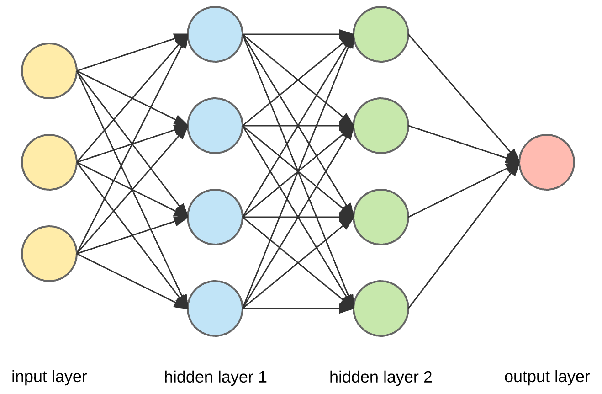
\includegraphics[width=4in]{dnn}
    % \caption[Struktura DNN - źródło: \url{https://towardsdatascience.com/building-a-convolutional-neural-network-male-vs-female-50347e2fa88b}]{Struktura DNN}
    \caption[Struktura DNN - źródło: \url{https://towardsdatascience.com}]{Struktura DNN}
    \label{fig:dnn}
  \end{figure}

  % Jedną z takich przełomowych architektur jest CNN (ang. convolutional neural
  % network). Są to sieci o hierarchicznej strukturze, gdzie obrazy wejściowe w
  % postaci macierzy wpier poddawane są ekstrakcji cech poprzez dokonanie operacji
  % konwolucji na obrazie poprzez przesuwanie zestawu filtrów wzdłuż obrazu.
  % Filtry te są zazywczaj inicjowane losowymi wartościami i w miarę trenowania,
  % dopasowują swoje parametry do wybranej problematyki.
  % Na wyjściu filtrów otrzymuje się macierze o mniejszej rozdzielczości
  % reprezentujące wyniki operacji konwolucji w danym punkcie. Otrzymane macierze
  % wyjściowe mogą być podawane na kolejne warstwy konwolucyjne w celu ekstrakcji
  % kolejnych cech. Dzięki temu procesowi kolejne warstwy filtrów uczą się
  % rozpoznawać kluczowe cechy na obrazie, od drobnych elemtów takich jak
  % krawędzie albo kształty po bardziej złożone takie jak części ciała albo
  % przedmioty.
  % Końcowe warstwy dokonują spłaszczania, czyli zamieniania wielowymiarowych
  % macierzy cech na jednowymiarowe wektore, które podawane są na wejście
  % FCL (ang. fully connected layer).

  % Lata rozwoju sztucznych sieci neuronowych zaowocowały powstaniem wielu technik służących do analizy i edycji obrazów. W poniższym rozdziale zaprezentowane zostaną, oraz pokrótce opisane, najważniejsze i najciekawsze przykłady, z których część znajdzie rozwinięcie w dalszej części tej pracy.

  \subsection{Sieci splotowe}
    \label{sieci_splotowe}

    Neuronowe sieci splotowe (CNN ang. convolutional neural network) stanowią podstawową strukturę w zakresie przetwarzania i analizowania obrazów cyfrowych. Są to sieci o hierarchicznej strukturze stanowiące podwaliny większości klasyfikatorów, detektorów, czy sieci segmentujących.

    Autorzy jednego z artykułów traktujących o sieciach splotowych \cite{cnn} opisują je następująco:
    \begin{quote}
      'CNN to skuteczny algorytm poznawczy, stosowany powszechnie przy rozpoznawaniu wzorców i przetwarzaniu obrazów. Posiada wiele cech, takich jak prosta struktura, mniej parametrów treningowych, czy zdolność do adaptacji. CNN stały się gorącym tematem w zakresie analizy głosu i rozpoznawania obrazu. Ich struktura oparta na podziale wag czyni je bardziej podobnymi do biologicznych sieci neuronowych. Redukuje to złożoność modelu sieci oraz liczbę wag'.
    \end{quote}

    Na CNN składają się zazwyczaj trzy rodzaje warstw, z których każda posiada inne cechy.

    Podstawową warstwę stanowi warstwa splotowa. Składa się ona ze zbioru filtrów (neuronów) odpowiedzialnych za ekstrakcję cech z analizowanych obrazów poprzez dokonanie operacji
    konwolucji na obrazie poprzez przesuwanie zestawu filtrów wzdłuż niego.
    Na wyjściu filtrów otrzymuje się macierze o mniejszej rozdzielczości
    reprezentujące wyniki operacji konwolucji w danym punkcie. Każda kolejna warstwa splotowa wydobywa z obrazu cechy o wyższych poziomach abstrakcji
    bazując na wynikach obliczeń poprzednich warstw tego rodzaju. Dzięki temu
    procesowi kolejne warstwy filtrów uczą się
    rozpoznawać kluczowe cechy na obrazie, od drobnych elementów takich jak
    krawędzie albo kształty po bardziej złożone takie jak części ciała albo
    całe obiekty. Filtry te są zazwyczaj inicjowane losowymi wartościami i w miarę trenowania, dopasowują swoje parametry do wybranej problematyki.

    Drugim istotnym elementem sieci splotowych jest warstwa poolingu. Może zostać opisana następująco \cite{deeplearn}:
    \begin{quote}
      'We wszystkich przypadkach pooling pomaga uczynić reprezentację w przybliżeniu niezmienną w stosunku do małych tłumaczeń danych wejściowych. Niezmienność wobec tłumaczenia oznacza, że jeśli poddamy dane wejściowe nieznacznej translacji, to wartość większości wyników poddanych poolingowi nie ulegnie zmianie'.
    \end{quote}

    Końcowy element CNN w większości przypadków stanowią warstwy gęste (FCL ang. Fully Connected Layer). Odpowiadają one za dokonanie odpowiedniej klasyfikacji obrazu na podstawie danych dostarczonych przez warstwy poprzedzające. Są przez to nieodzowne w przypadku zadań związanych z wszelkiego rodzaju klasyfikacją obrazów.

    Wymienione tutaj elementy składowe sieci splotowych mogą przyjmować różne rozmiary i występować w różnych konfiguracjach, co przedstawiono na poniższym Rysunku \ref{fig:cnn_structure}.
    \begin{figure}[h]
     \centering
     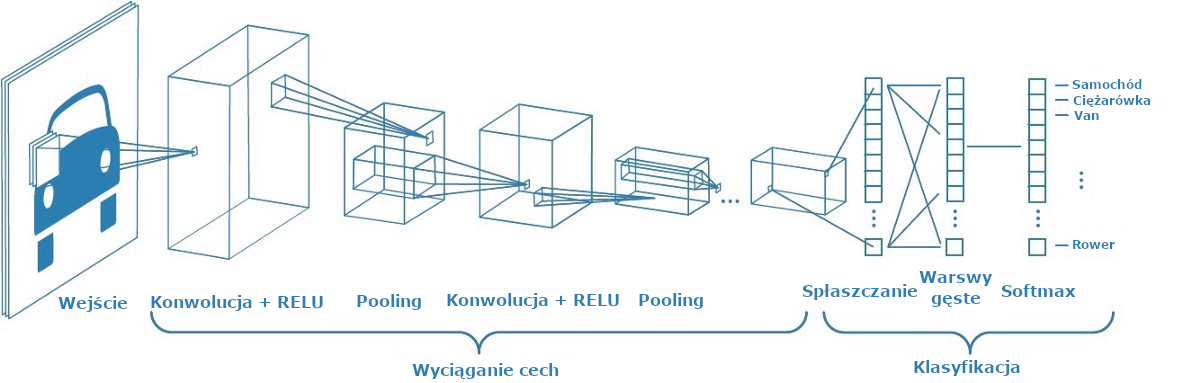
\includegraphics[width=4in]{cnn_structure}
     % \caption[Przykładowa struktura CNN - źródło: \url{https://www.mathworks.com/solutions/deep-learning/convolutional-neural-network.html}]{Przykładowa struktura CNN}
     \caption[Przykładowa struktura CNN - źródło: \url{https://www.mathworks.com}]{Przykładowa struktura CNN}
     \label{fig:cnn_structure}
    \end{figure}
    \newline
    Zapewnia to szerokie pole do eksperymentów i sprawia, że sieci te zdolne są rozwiązywać złożone, różnorodne problemy z wielu dziedzin codziennego życia.

  \subsection{FCN}

   Jednym z kluczowych problemów, jakie stawia przed badaczami edycja obrazów jest zagadnienie segmentacji semantycznej. Klasyczna klasyfikacja, polegająca na przypisywaniu obrazów do odpowiednich grup tematycznych, jest w tym przypadku sprowadzana do poziomu pojedynczych pikseli. Oznacza to, że sieci neuronowe przeznaczone do tego zadania są w stanie dokonać klasyfikacji dla każdego pojedynczego piksela analizowanego obrazu. Na tej podstawie uzyskiwany jest podział na segmenty, z których każdy reprezentuje inną klasę obiektów, jak na poniższym Rysunku \ref{fig:segmentation}.

   \begin{figure}[h]
    \centering
    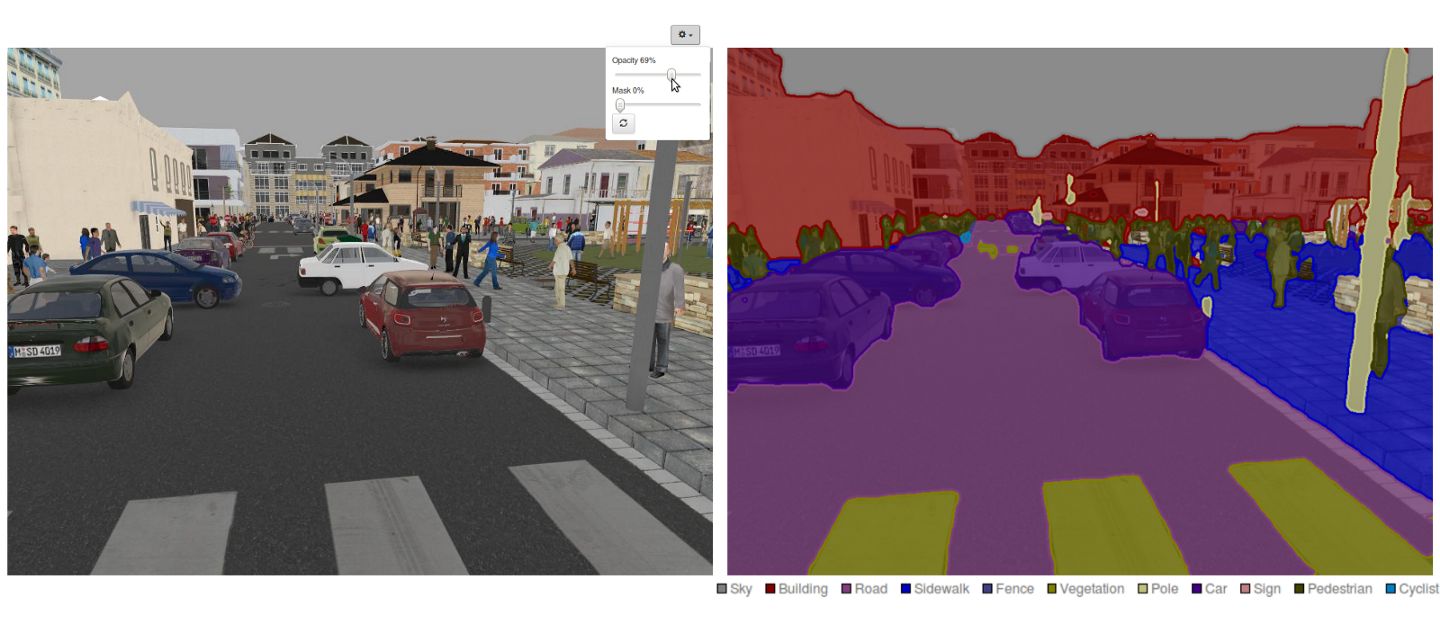
\includegraphics[width=4in]{segmentation}
    % \caption[Segmentacja semantyczna - źródło: \url{https://devblogs.nvidia.com/image-segmentation-using-digits-5/}]{Segmentacja semantyczna}
    \caption[Segmentacja semantyczna - źródło: \url{https://devblogs.nvidia.com}]{Segmentacja semantyczna}
    \label{fig:segmentation}
  \end{figure}

   W większości modele odpowiadające za przeprowadzanie segmentacji składają się z szeregowego połączenia enkodera oraz dekodera. Enkoder jest zazwyczaj pre-trenowaną siecią neuronową przeznaczoną do klasyfikowania obrazów. Dekoder odpowiada za semantyczne rzutowanie cech w niskiej rozdzielczości, wyuczonych przez enkoder, na wysoką rozdzielczość samych pikseli tworząc wspomniany wcześniej podział segmentowy.

   FCN (ang. Fully Convolutional Networks) stanowią szczególny rodzaj sieci neuronowych przeznaczonych do segmentacji obrazów. Składają się one wyłącznie z kombinacji warstw splotowych oraz poolingu. Są w stanie przetwarzać obrazy o dowolnej, zmiennej wielkości, w odróżnieniu od innych typów modeli, w których zastosowanie warstw gęstych (FCL) wymusza z góry ustalone rozmiary danych wejściowych.

   Naprzemienne przepuszczanie obrazów przez wspomniane warstwy splotowe oraz pooling może powodować niską rozdzielczość wyjściowych rezultatów pracy tych sieci oraz rozmycie granic poszczególnych obiektów. Z tego powodu w nowoczesnych rozwiązaniach stosuje się dodatkowe mechanizmy zapobiegające tego typu trendom.

  \subsection{Modele generatywne}
  \label{modele_generatywne}
   Koncepcja modeli generatywnych, w skrócie GANów, przedstawiona została w 2014 roku przez Iana Goodfellow oraz jego współpracowników na uniwersytecie w Montrealu \cite{gan}. Modele te stanowią połączenie dwóch głębokich sieci neuronowych działających przeciwstawnie do siebie nawzajem.

   Pierwsza sieć to tak zwany generator. W odniesieniu do tematu pracy, jego działanie polega na generowaniu nowych obrazów, lub ich fragmentów na podstawie wektora szumów.

   Obrazy te przekazywane są, równolegle z zestawem obrazów prawdziwych, do dyskryminatora stanowiącego drugą część modelu GAN. Działanie tej sieci neuronowej polega na określeniu (w skali 0 do 1), w jakim stopniu produkty wyjściowe generatora odpowiadają obrazom rzeczywistym.

   W opisanym modelu występuje zatem podwójna pętla sprzężenia zwrotnego. Dyskryminator określa autentyczność obrazów porównując je ze zdefiniowaną odgórnie bazą danych. Z kolei generator otrzymuje informację o skuteczności swojego działania ze strony dyskryminatora.

   Model generatywny znajduje się w stanie ciągłego konfliktu. Generator dąży do jak najdokładniejszego fałszowania obrazów w celu oszukania dyskryminatora, którego celem jest z kolei jak najdokładniejsze wykrywanie podróbek. Obie sieci neuronowe nieustannie dążą do osiągnięcia przewagi nad rywalem w procesie treningu. Ciągła rywalizacja sprawia, że zarówno generator, jak i dyskryminator zyskują coraz wyższą skuteczność działania.

   W praktyce modele generatywne są w stanie naśladować dowolną dystrybucję danych. Są w stanie kreować światy podobne do naszego w zakresie obrazu, dźwięku czy mowy. Można powiedzieć, że są to prawdziwi syntetyczni artyści.


\section[Przegląd rozwiązań (Bartosz Bieliński)]{Przegląd rozwiązań}

  Na przestrzeni ostatnich paru lat pojawiło się wiele innowacyjnych technologii opartych
  na sieciach neuronowych. Takie cechy sieci, jak niezwykłe zdolności do generalizacji
  zdobytej wiedzy na nowe przypadki oraz olbrzymia elastyczność sprawiły, że
  znalazły one wiele rzeczywistych zastosowań, zwłaszcza do problemów
  nieszablonowych, dla których metody nie oparte na uczeniu maszynowym
  nie przynosiły zadowalających wyników. Zastosowania te często były
  przełomowe w swojej dziedzinie i do czasów dzisiejszych uważane są
  za prekursorów pewnych idei.

  W tym rozdziale skupiono się na przedstawieniu kilku interesujących rozwiązań
  stosujących sieci neuronowe do edycji obrazu, które są zarazem kluczowe do lepszego
  zapoznania się z omawianą problematyką.

  \subsection{Colorful image colorization}

    Wraz z rozwojem sieci neuronowych, rosło zainteresowanie możliwościami zastosowania
    ich do kolorowania czarno-białych obrazów. Jedno z dostępnych rozwiązań tego
    zagadnienia zostało przedstawione przez grupę pracowników Uniwersytetu w
    Berkeley \cite{colorful_image_colorization}. Celem ich pracy było stworzenie
    modelu, który niekoniecznie odtwarza oryginalne barwy obrazu, ale generuje
    barwy prawdopodobne, zdolne przekonać ludzkiego obserwatora o autentyczności
    obrazu. Uzyskane rezultaty zostały przedstawione na
    Rysunku \ref{fig:colorful_image_colorization}.

    \begin{figure}[ht]
      \centering
      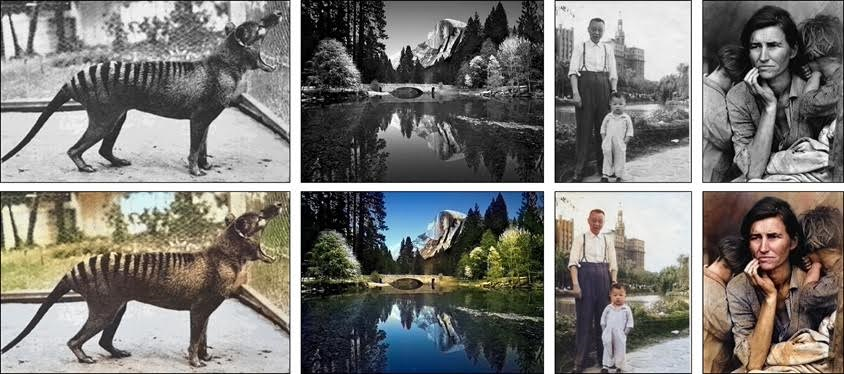
\includegraphics[width=4in]{image_colorization}
      \caption[Efekt kolorowanie czarno-białych obrazów przez wytrenowany model - źródło:
      \cite{colorful_image_colorization}]{Efekt kolorowanie czarno-białych obrazów przez wytrenowany model.}
      \label{fig:colorful_image_colorization}
    \end{figure}

    Wykorzystany model składa się z wielu warstw CNN, w których skład wchodzą
    warstwa filtrów konwolucyjnych, warstwa ReLU (ang. Rectified
    Linear Unit) oraz warstwa BatchNorm (ang. Batch normalization).
    Aby zapobiec utracie informacji przestrzennych, sieć nie posiada warstw poolingu.
    Istotny był także sposób
    przygotowania zbioru danych do trenowania modelu. Obrazy ze zbioru uczącego
    były wpierw konwertowane do modelu barw YUV. Kanał Y był podawany na
    wejście sieci, a kanały UV pełniły funkcję pożądanej odpowiedzi w uczeniu
    nadzorowanym.

    Ważnym aspektem zbadanym w artykule było także dobranie odpowiedniej
    funkcji kosztu. Nieodpowiedni wybór skutkował desaturacją kolorowanych
    obrazów. Jedną z potencjalnych przyczyn tego zjawiska może być tendencja
    sieci do tworzenia bardziej konserwatywnych odpowiedzi. Aby zniwelować ten
    efekt, w modelu została zastosowana specjalna technika modyfikacji
    funkcji kosztu. Polega ona na przewidywaniu dystrybucji możliwych kolorów
    dla każdego piksela i poprawie wartości wyliczanego dla modelu błędu, w celu
    wyróżnienia rzadko spotykanych kolorów.

    Powstałe rozwiązanie dowodzi olbrzymiego potencjału zastosowania sieci
    neuronowych w dziedzinie pracy nad obrazami, efekty uzyskiwane za ich pomocą
    są niemożliwe do odtworzenia z użyciem tradycyjnych algorytmów.

  \subsection{Image Style Transfer Using Convolutional Neural Networks}

    W roku 2016 został przedstawiony światu \textit{A Neural Algorithm of Artistic Style}
    \cite{image_style_transfer}. Wprowadzał on przełom w dziedzinie przenoszenia
    stylu jednego obrazu na inny, a jego sukces opierał się na właściwym wykorzystaniu
    konwolucyjnych sieci neuronowych. Podstawą tego osiągnięcia było odkrycie przez
    Leona A. Gatys oraz jego współpracowników, że w CNN reprezentacja treści
    obrazu oraz jego stylu jest rozłączna. Umożliwia to wydobycie stylu
    przetwarzanego obrazu oraz połączenie go z treścią innego obrazu, czego
    dokonuje właśnie \textit{A Neural Algorithm of Artistic Style}. Rezultaty takich
    operacji można zaobserwować na Rysunku \ref{fig:image_style_transfer}

    \begin{figure}[H]
      \centering
      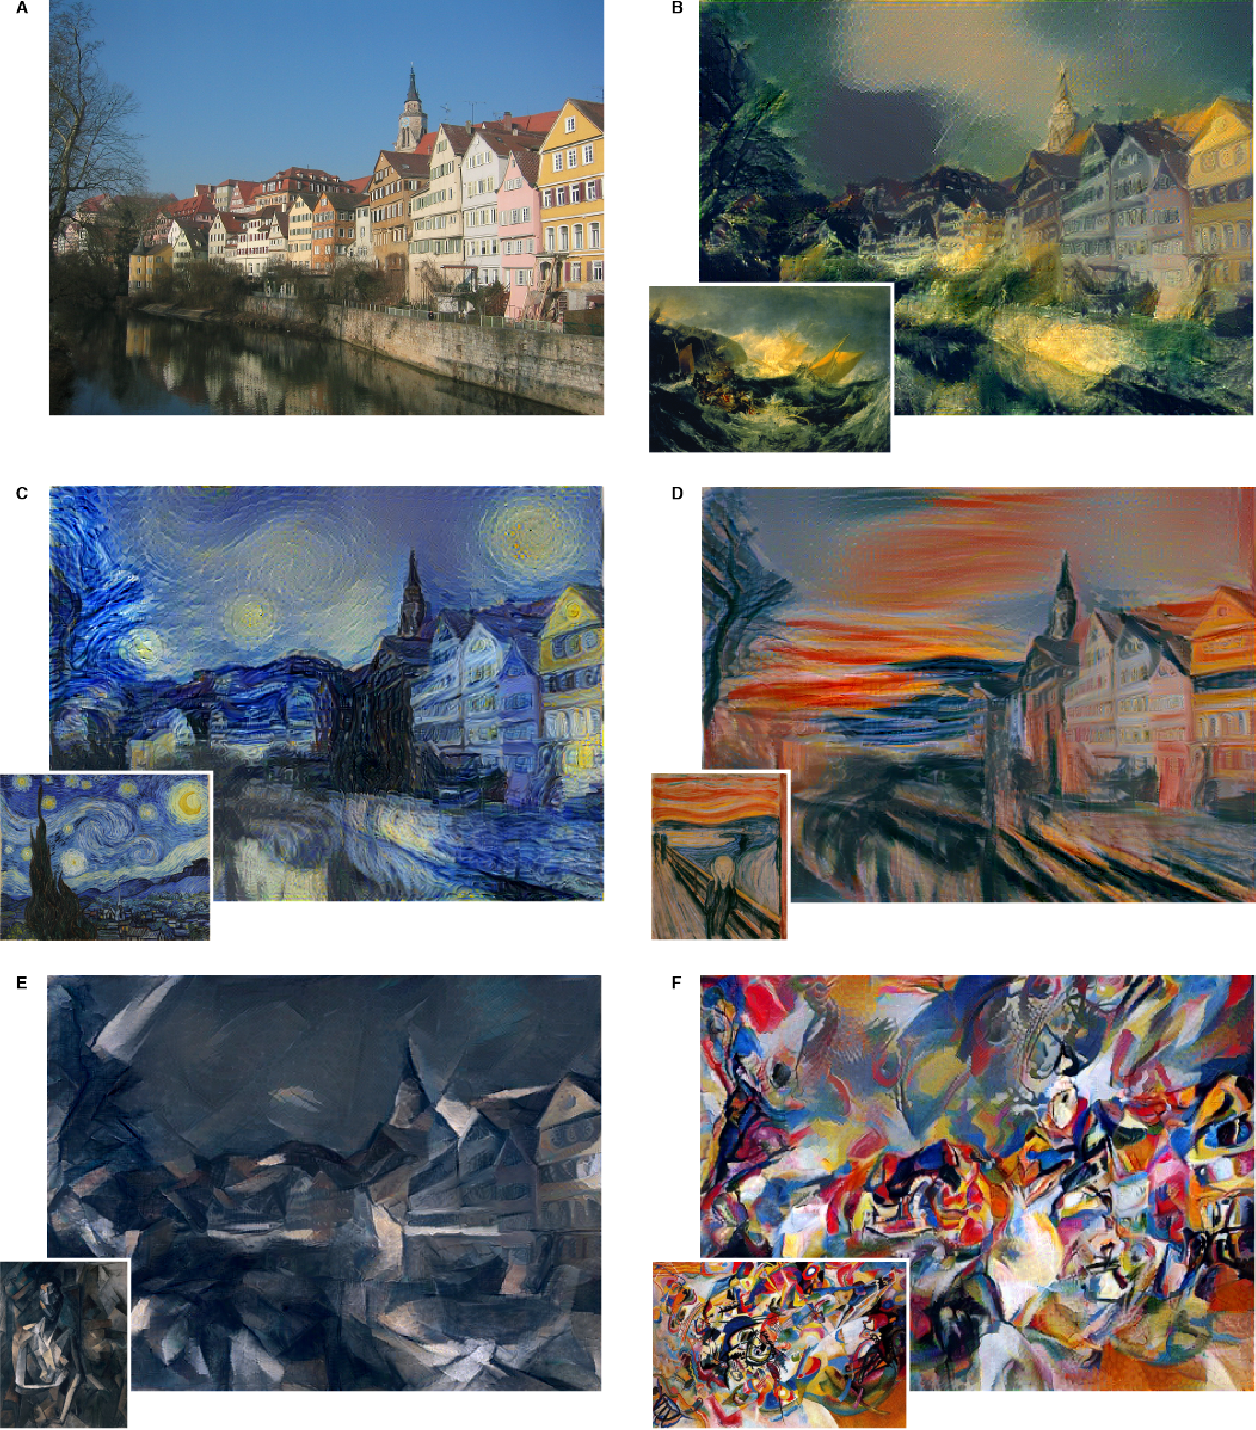
\includegraphics[width=4in]{image_style_transfer}
      \caption[Obrazy będące kombinacją treści zdjęcia ze stylami kilku znanych dzieł sztuki - źródło:
      \cite{image_style_transfer}]
      {Obrazy będące kombinacją treści zdjęcia ze stylami kilku znanych dzieł sztuki.}
      \label{fig:image_style_transfer}
    \end{figure}

    Do zbudowania modelu zostały użyte warstwy konwolucyjne oraz poolingu z
    architektury VGG-Network \cite{vgg_network}, która została wytrenowana pod
    kątem rozpoznawania obiektów i określania ich położenia. Dzięki temu sieć
    przetwarzając obraz tworzy jego reprezentację, która wraz z
    kolejnymi warstwami, przedstawia coraz pełniejszą informację o obiektach,
    a niekoniecznie o dokładnym wyglądzie obrazu.
    W modelu nie została użyta ani jedna warstwa gęsta, dzięki czemu na wyjściu
    możliwe jest otrzymanie dwuwymiarowego obrazu.
    Dla lepszej syntezy obrazów, w warstwach
    łączących zastosowano próbkowanie wartością średnią, zamiast najczęściej
    stosowaną wartością maksymalną.
    Takie zabiegi umożliwiają wyliczenie reprezentacji stylu z korelacji
    pomiędzy poszczególnymi cechami w kolejnych warstwach konwolucyjnych.

    Cały proces renderowania polega na odpowiednim przechowaniu w modelu treści
    oraz stylu wejściowych obrazów i składa się z wielu następujących po sobie etapów.
    Wpierw obraz, z którego pobierany jest styl, jest podawany na
    wejście sieci oraz przetwarzany, reprezentacja stylu, wyselekcjonowana z
    właściwych warstw, jest odpowiednio przechowywana. Następnie temu samemu
    procesowi poddawany jest obraz z treścią, ale reprezentacja treści jest wyciągana z ostatnich
    warstw konwolucyjnych.
    W celu wykonania fuzji obrazów, uzyskane reprezentacje treści oraz stylu są
    zapisywane w tych warstwach modelu skąd zostały odczytane, po czym na wejście
    podawany jest obraz składający się z losowego szumu białego.
    Następnie, poprzez iteracyjną minimalizację funkcji kosztu, obraz wejściowy jest modyfikowany, co w rezultacie końcowym doprowadza do nałożenia zapisanego
    stylu na wczytaną treść.

    \textit{A Neural Algorithm of Artistic Style} jest świetnym przykładem, jak elastyczne
    mogą być interfejsy do modyfikacji obrazu oparte na technologii sieci neuronowych.

  \subsection{Invertible Conditional GANs for image editing}
    Edycja obrazów może być dokonywana na wielu różnych poziomach zaawansowania
    i abstrakcji, operacje niezłożone, takie jak nakładanie filtrów, mogą być
    wykonywane przez proste algorytmy. Jednak w przypadku próby modyfikacji
    elementów na obrazie, algorytmy te nie będą w stanie dokonać semantycznych
    zmian, ze względu na brak możliwości zrozumienia treści obrazu. Rozwiązanie
    tego problemu zostało przedstawione w postaci modelu IcGAN
    (ang. Invertible conditional Generative Adversarial Network) w roku 2016
    \cite{gan_editing}. Zaprezentowany model to enkoder z możliwością
    generowania wektora informacji o atrybutach obrazu, połączony z warunkowym
    GANem zdolnym do kontrolowania cech generowanych obrazów na podstawie dodatkowej
    informacji warunkowej. Takie działanie umożliwia wprowadzanie zmian w
    atrybutach generowanego obrazu uzyskiwanego na wyjściu cGAN (ang. conditional Generative
    Adversarial Network). Rezultaty działania modelu można zaobserwować na
    Rysunku \ref{fig:IcGAN}

    \begin{figure}[ht]
      \centering
      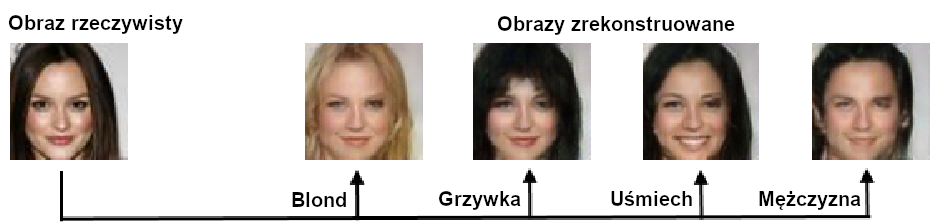
\includegraphics[width=4in]{IcGAN}
      \caption[Obrazy generowane przez IcGAN - źródło: \cite{gan_editing}]{Obrazy generowane przez IcGAN.}
      \label{fig:IcGAN}
    \end{figure}

    Wykorzystany w IcGAN ekonder w rzeczywistości składa się z dwóch podrzędnych
    enkoderów. Enkoder $E_{z}$ koduje wejściowy obraz do utajonego wektora $z$ reprezentacji
    obrazu, natomiast enkoder $E_{y}$ generuje wektor informacji $y$, oddający
    pewne kluczowe atrybuty obrazu. Enkodery są trenowane z użyciem już wytrenowanego
    cGAN oraz obrazów rzeczywistych z etykietami ze zbioru uczącego. Zbadane
    zostały także różne podejścia interakcji między dwoma enkoderami, wyróżnić
    można podejście, w którym enkodery są w pełni niezależne, podejście
    gdzie wyjście $E_{z}$ jest zależne od wyjścia $E_{y}$, a także podejście
    gdzie $E_{z}$ oraz $E_{y}$ są połączone w jeden enkoder o współdzielonych
    warstwach i dwóch wyjściach.

    W przypadku cGAN można wyróżnić dwa najważniejsze czynniki, które trzeba
    mieć na uwadze. Pierwszym jest źródło wektora $y$ podawanego na
    generator. W przypadku dyskryminatora, $y$ jest pobierany ze
    zbioru treningowego, jednakże w przypadku podawania tego
    samego wektora na generator, pojawia się możliwość wystąpienia niepożądanego
    przeuczenia modelu. Autorzy artykułu dokonali analizy tego rozwiązania,
    a także zbadali wydajność metod Bezpośredniej Interpolacji oraz
    Jądrowego Estymatora Gęstości. Wynikiem tych badań było stwierdzenie, że
    dla danej problematyki najlepiej sprawdza się podawanie wektora $y$ ze zbioru
    uczącego. Możliwość przeuczenia modelu została skomentowana następująco:
    \begin{quote}
      % This is only likely to occur if the conditional information
      % is, to some extent, unique for each image. In the case where the attributes of an image are binary, one attribute vector y could describe a varied and large enough subset of images, preventing the model from overfitting given y.
      'Jest to możliwe tylko, gdy informacje warunkowe są do pewnego stopnia
      unikatowa dla każdego obrazu. W tym przypadku, gdzie atrybuty obrazów są
      binarne, jeden wektor $y$ może opisać wystarczająco duży i zróżnicowany
      podzbiór obrazów, zapobiegając nadmiernemu dopasowaniu się modelu do
      danego $y$.'
    \end{quote}

    Drugim czynnikiem jest warstwa generatora i dyskryminatora cGAN na
    którą podany jest wektor $y$. Guim Perarnau oraz jego współpracownicy ustalili, że najlepsze rezultaty otrzymuje się po podaniu wektora $y$ na warstwę wejściową
    generatora oraz pierwszą warstwę konwolucyjną dyskryminatora.

    Ważnym spostrzeżeniem z analizy rozwiązania IcGAN jest obecność
    olbrzymiej liczby różnorodnych rozwiązań opartych na sieciach neuronowych.
    Coraz to nowe architektury zostają wynalezione, aby udoskonalić
    zastosowania sieci neuronowych do przetwarzania i modyfikowania obrazów.

  \subsection{Neural photo editing}
    W 2017 roku Andrew Brock, Theodore Lim, J.M. Ritchie and Nick Weston
    zaprezentowali \textit{Neural Photo Editor} \cite{neural_photo_editor}, narzędzie
    do edytowania obrazu wyposażone w mechanizmy wykrywania kontekstu zmiany.
    Twórcy opisują swoje dzieło następująco:

    \begin{quote}
      % 'An interface that leverages the power of generative neural networks to
      % make large, semantically coherent changes to existing images.'
      'Interfejs wykorzystujący moc generatywnych sieci neuronowych do
      wprowadzania dużych, semantycznie spójnych zmian w istniejących obrazach.'
    \end{quote}

    Użytkowanie wygląda następująco: użytkownik pędzlem o określonym kolorze i
    rozmiarze maluje na wybranym obrazie, jednak zamiast zmieniać wartości
    pojedynczych pikseli, interfejs odczytuje kontekst wprowadzanej edycji.
    Następnie na jego podstawie wprowadza zmiany
    semantyczne w kontekście żądanej zmiany koloru. Efekt działania interfejsu
    został przedstawiony na Rysunku \ref{fig:npe}.

    \begin{figure}[ht]
      \centering
      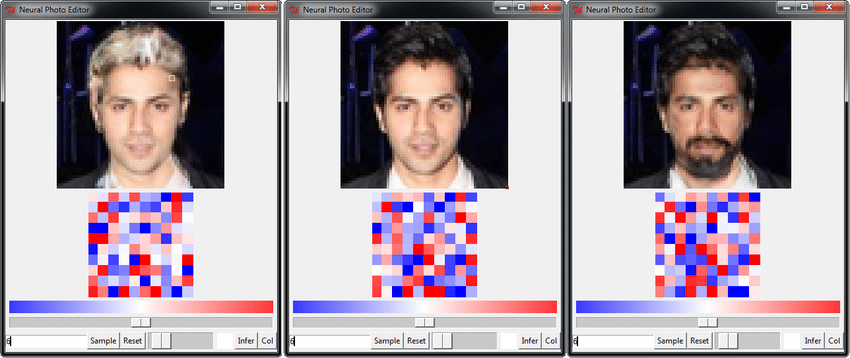
\includegraphics[width=4in]{NPE}
      \caption[Efekt działania \textit{Neural Photo Editor} - źródło: \cite{neural_photo_editor}]
      {Efekt działania Neural Photo Editor.}
      \label{fig:npe}
    \end{figure}

    Skuteczność NPE (ang. Neural Photo Editor) polega na zastosowaniu IAN
    (ang. Introspective Adversarial Network), czyli sieci złożonej z połączonych
    VAE (ang. Variational Autoencoder) \cite{vae} oraz GANów, w taki sposób, że dekodująca
    sieć autoenkodera jest używana jako sieć generująca w GANie.
    Poprzez przechwytywanie przez model dalekosiężnych zależności, wykorzystanie
    bloku obliczeniowego bazującego na rozszerzonych splotach o
    współdzielonych wagach oraz dzięki zastosowaniu ulepszonej generalizacji,
    udało się osiągnąć dokładną rekonstrukcję obrazu bez strat na jakości detali.

    Powstanie NPE utwierdza w przekonaniu, że aktualnie istniejące sieci
    neuronowe do edycji obrazu znacznie przewyższają zwykłe algorytmy pod
    względem możliwości, a także są zauważalnie słabiej uzależnienie od wkładu
    ludzkiego.


\section{Zaimplementowane rozwiązania}

  W celu zbadania skuteczności sieci neuronowych jako narzędzi do edycji obrazu
  należało wybrać przykładowe zagadnienia z tej dziedziny, rozwiązać je z
  użyciem technik sztucznej inteligencji oraz ocenić ich skuteczność.

  W tym rozdziale zostały przedstawione koncepcje rozwiązań wybranych zagadnień
  oraz ich implementacje.

  \subsection{Automatyczne kolorowanie czarno-białych obrazów}

  Problem kolorowania czarno-białych obrazów cieszy się dużym zainteresowaniem z
  wielu powodów. Od potrzeb kulturowych takich jak możliwość lepszego
  zwizualizowania oraz zrozumienia przeszłości poprzez kolorowania zdjęć z
  czasów, kiedy występowały one jedynie w kolorach czerni i bieli, po potrzeby
  technologiczne takie jak rekonstrukcja filmów oraz poprawa obrazu cyfrowego.

  Pomimo braku informacji o kolorze w czarno-białych zdjęciach, ludzie są w
  stanie określić potencjalne, rzeczywiste barwy obiektów na zdjęciach bazując
  na treści tych zdjęć oraz swoim doświadczeniu. Można z tego wywnioskować, że
  zdjęcia te zawierają informacje wystarczające do oszacowania potencjalnych
  kolorów. Pozwala to założyć, że do tego zagadnienia można skutecznie wykorzystać
  konwolucyjne sieci neuronowe, które cechują się niezwykłą umiejętnością do
  rozpoznawania wzorców oraz posiadają wyjątkowe zdolności do adaptacji. Z tego
  właśnie powodu sieci splotowe zostaną użyte w przedstawionym rozwiązaniu.

\subsubsection{Podejście}

  Rozważając możliwe sposoby pokolorowania czarno-białego zdjęcia można spostrzec,
  że kiedy niektóre powierzchnie na zdjęciu mają zazwyczaj oczywiste barwy, niebo
  jest zazwyczaj niebieskie, a trawa zielona, to są też powierzchnie, które
  posiadają szeroki wachlarz możliwych kolorów, na przykład samochodów może być
  zarówno czerwony jak i niebieski albo zielony. Z tego powodu celem zaprezentowanego
  rozwiązania jest niekoniecznie odtworzenie rzeczywistych barw obrazu, a raczej
  wygenerowanie barw, które mogłyby być barwami rzeczywistymi.

  Aby zwiększyć efektywność uczenia wykorzystano przestrzeń barw CIELab. W tej
  przestrzeni barwę obrazu opisują 3 składowe:
  \begin{itemize}
  \item L - jasność (luminacja)
  \item A - barwa od zielonej do magenty
  \item B - barwa od niebieskiej do żółtej
  \end{itemize}
  Przestrzeń barw CIELab została przedstawiona na Rysunku \ref{fig:CIELab}

  \begin{figure}
    \centering
    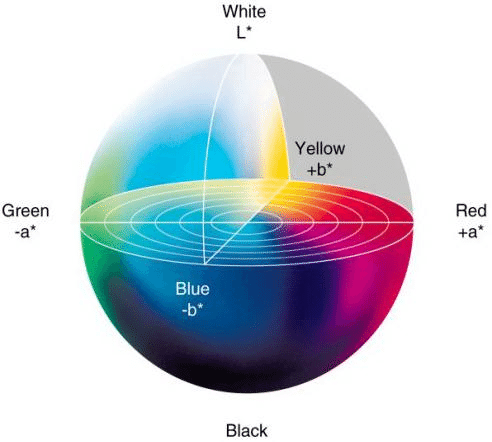
\includegraphics[width=3.5in]{CIELab}
    \caption[Przestrzeń barw CIELab - źródło:
    \url{https://www.flickr.com/photos/greenmambagreenmamba/4236391637}]
    {Przestrzeń barw CIELab.}
    \label{fig:CIELab}
  \end{figure}

  Zaletą zastosowania CIELab jest fakt, że jest ona najbardziej równomierną
  przestrzenią barw, co oznacza, że jeśli barwy znajdują się w jednakowej
  odległości od siebie w tej przestrzeni, to będą one postrzegane jako jednakowo
  różniące się od siebie. Powinno to zwiększyć skuteczność uczenia sieci oraz
  zapewnić bardziej realistyczne kolorowanie.

  Składowa \textit{L}, jako, że jest identyczna dla obrazu kolorowego jak i
  czarno-białego, stanowi w tym przypadku wejście sieci, na jej podstawie sieć
  odtwarza składowe \textit{A} oraz \textit{B}, które reprezentują przewidziane
  kolory dla obrazu wejściowego. W celu lepszego zrozumienia formatu przykładowa
  składowa \textit{L} została przedstawiona na Rysunku \ref{fig:przyklad_L}.
  Jak widać zawiera ona informacje wystarczające do rozróżnienia między sobą
  powierzchni oraz wydobycia ich kluczowych cech.

  \begin{figure}[ht]
    \centering
    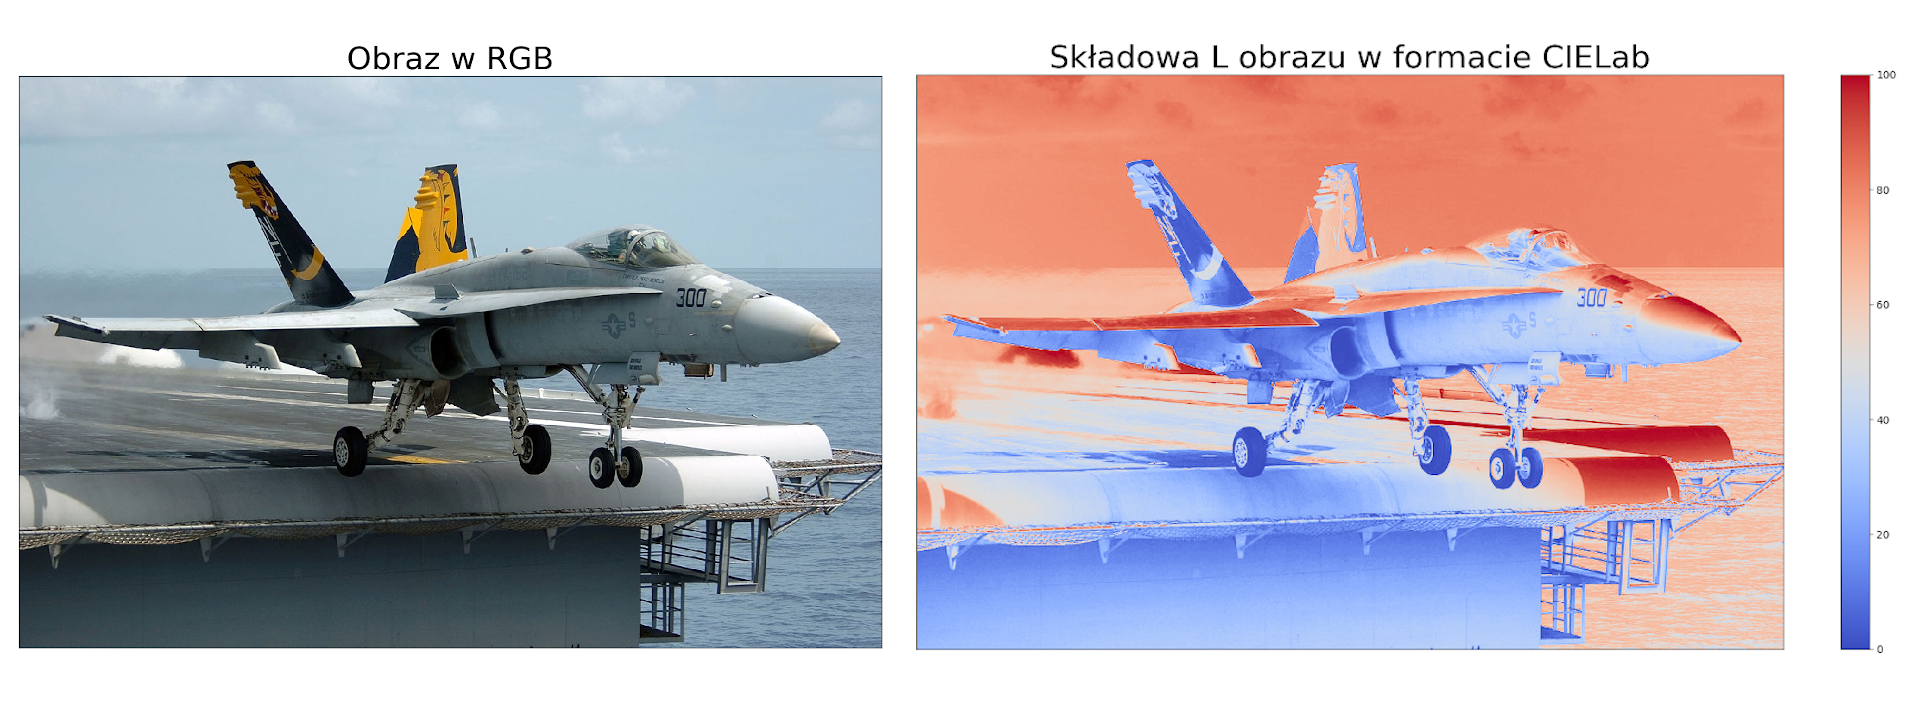
\includegraphics[width=6in]{rgb_i_L}
    \caption[Przykładowa składowa \textit{L} - źródło: Rysunek własny
    wykorzystujący:
    \url{https://fr.m.wikipedia.org/wiki/Fichier:An_F-A-18C_Hornet_launches_from_the_flight_deck_of_the_conventionally_powered_aircraft_carrier.jpg}]
    {Przykładowa składowa \textit{L}.}
    \label{fig:przyklad_L}
  \end{figure}

  Jako rozwiązanie podanej problematyki wpierw został oceniony autorski
  model, na jego podstawie zostało przeprowadzone porównanie skuteczności
  różnych konfiguracji, w których uczony był model. Do elementów poddanych
  testom należą algorytm optymalizacyjny, funkcja straty, funkcja aktywacja oraz
  sposób przetwarzania wstępnego danych treningowych.

\subsubsection{Model końcowy}

  Opracowany przez nas model jest to FCN. Konwolucyjna część sieci składa się
  z 12 warstw splotowych
  mających na celu nauczyć się mapować składową wejściową \textit{L} na wyjściowe
  składowe \textit{A} i \textit{B}. Składowe wyjściowe muszą mieć takie same
  wymiary jak składowa wejściowe, co oznacza, że kluczowym było odpowiednie dobranie
  parametrów warstw takich jak \textit{padding} (pol. otoczka), \textit{stride}
  (pol. krok) oraz wielkość filtrów. Pełna architektura sieci została przedstawiona w
  Tabeli \ref{table:model_architecture}.
  \noindent\begin{table}[H]
    \center
    \begin{tabular}{|c | c | m{3.3em} | c | c | m{4em} | c | c| }
     \hline
     Nr & Warstwa & Rozmiar filtra & Stride & Padding & Batch Normalization &
     Fun. aktywacji & Ilość kanałów wej./wyj. \\ [0.5ex]
    \hline
    1 & Splotowa & 3x3 & 1 & 1 & Tak & ReLU & 1/32 \\ \hline
    2 & Splotowa & 3x3 & 1 & 1 & Tak & ReLU & 32/32 \\ \hline
    3 & Splotowa & 3x3 & 1 & 1 & Tak & ReLU & 32/32 \\ \hline
    4 & Splotowa & 3x3 & 1 & 1 & Tak & ReLU & 32/32 \\ \hline
    5 & Splotowa & 3x3 & 1 & 1 & Tak & ReLU & 32/64 \\ \hline
    6 & Splotowa & 3x3 & 1 & 1 & Tak & ReLU & 64/64 \\ \hline
    7 & Splotowa & 3x3 & 1 & 1 & Tak & ReLU & 64/64 \\ \hline
    8 & Splotowa & 3x3 & 1 & 1 & Tak & ReLU & 64/32 \\ \hline
    9 & Splotowa & 3x3 & 1 & 1 & Tak & ReLU & 32/32 \\ \hline
    10 & Splotowa & 1x1 & 1 & 0 & Tak & ReLU & 32/32 \\ \hline
    11 & Splotowa & 1x1 & 1 & 0 & Tak & ReLU & 32/32 \\ \hline
    12 & Splotowa & 1x1 & 1 & 0 & Nie & - & 32/2 \\ \hline
    \end{tabular}
    \caption{Architektura modelu podstawowego.}
    \label{table:model_architecture}
  \end{table}
  Pierwsza warstwa konwolucyjna rozkłada wejściowy kanał na 32 kanały, co
  pozwala wyciągnąć z niego jak najwięcej informacji o cechach obrazu. Warstwa
  ta ma wielkość filtra 3x3, tak więc aby zachować wymiar kanałów zostały
  zastosowane parametry $\textit{padding}=1$ oraz $\textit{stride}=1$.

  Kolejne trzy warstwy ekstraktują z wejściowych 32 kanałów najbardziej istotne
  cechy związane z powiązaniem treści obrazu z szacowanym kolorem jego powierzchni.
  Warstwy te na swoje wyjście przekazują po 32 kanały zawierające wykryte
  powiązanie pomiędzy pikselami kanałów wejściowych.

  Warstwa piąta rozciąga wejściowe 32 kanały na 64 kanały, dzięki temu kolejne
  2 warstwy przyjmujące na wejście te 64 kanały i przekazujące je na wyjście są
  w stanie wydobyć z obrazu cechy o większym poziomie abstrakcji, co znacznie
  zwiększa skuteczność działania sieci.

  Warstwa ósma ogranicza ilość kanałów w sieci z 64 do 32 wyciągając z nich
  cechy najbardziej przydatne do rozwiązania danej problematyki. Kanały te są
  następnie ponownie przetwarzane przez warwę z wielkością filtru 3x3, co ma
  służyć agregacji rozłożonych cech w bardziej spójną całość, która może być
  już składana w pożądane wyjście.

  Kolejne dwie warstwy w sieci są to warstwy konwolucyjne o wielkości filtru 1x1,
  odpowiadają one warstwom gęstym i mają na celu przekonwertowanie wartości
  funkcji aktywacji z poprzednich warstw na wartości kolorów odpowiadających
  pikseli w przestrzeni barw CIELab. Ostatnia warstwa, również z filtrem o
  wielkości 1x1 zwija 32 kanały otrzymywane na wejściu do 2 kanałów odpowiadających
  składowym \textit{A} oraz \textit{B}, które stanowią pożądany rezultat działania
  sieci.

  Po wszystkich, oprócz ostatniej, warstwach konwolucyjnych znajdują się dodatkowo
  warstwa BatchNorm oraz warstwa funkcji aktywacji ReLU mające na celu
  ustabilizować proces uczenia oraz zwiększyć jego efektywność.

\subsubsection{BatchNorm} \label{BatchNorm}

  Warstwa Batch Normalization została przedstawiona w 2015 roku przez S. Ioeffe
  oraz C. Szegedy jako odpowiedź
  na problem zmieniającej się podczas uczenia dystrybucji wartości wejść
  każdej z warstw sieci \cite{BatchNorm}. Ma ona na celu usprawnić i ustabilizować
  trening sieci poprzez normalizację wartości podawanych na funkcje aktywacji.
  Zmienna dystrybucja tych wartości znacznie spowalnia i utrudnia proces uczenia
  poprzez potrzebę przemyślanego inicjowania
  wag sieci w celu zwiększenia prawdopodobieństwa nakierowania modelu na pożądane
  rozwiązania w trakcie procesu uczenia oraz przez
  konieczność używania mniejszych wartości współczynnika uczenia, aby
  przeciwdziałać problemom zanikającego oraz wybuchającego gradientu
  \cite{exploding_vanishing_grad}.

  Problemy te zostały już zauważone i opisane w 1994 roku przez Y. Bengio
  oraz jego współpracowników \cite{exploding_vanishing_grad}. Dowodzą oni, że:
  \begin{quote}
    % 'Gradient descent becomes increasingly inefficient when the
    % temporal span of the dependencies increases'
    'Metoda gradientu prostego staje się coraz bardziej nieefektywna, gdy
    rośnie czasowy zakres zależności'
  \end{quote}
  Wskazują także, że problemy powstają podczas treningu DNN w fazie wstecznej
  propagacji błędu, kiedy to gradient pochodzący z głębszych warstw przechodzi
  wielokrotnie przez operacje mnożenia macierzowego. Jeśli wartość gradientu
  jest niewielka, to z każdą operacją mnożenia staje się jeszcze mniejsza, aż
  maleje do takich wartości, które nie umożliwiają modelowi uczenia się, a jeśli
  wartość ta jest wysoka to, wraz z przechodzeniem przez kolejne warstwy, rośnie
  jeszcze bardziej co przy bardzo dużych wartościach może doprowadzić do
  destabilizacji procesu uczenia. Są to zjawiska zdecydowanie niepożądane i z
  tego powodu powstało wiele rozwiązań, aby im przeciwdziałać takich jak
  ograniczanie maksymalnej wartości gradientu (ang. gradient clipping) albo
  zastosowanie warstw BatchNorm.

  Zastosowanie warstw BatchNorm sprawia, że podczas uczenia metodą mini-batch
  (pol. małych paczek) każda paczka jest
  normalizowana w sposób zapewniający zerową wartość średnią oraz
  równą jedności wariancję na przestrzeni wszystkich kanałów wejściowych.
  Zaletą takiego podejścia jest poprawienie przepływu korygującego gradientu
  przez kolejne warstwy sieci podczas fazy wstecznej propagacji błędu. Ponadto
  warstwy BatchNorm zapewniają większą odporność sieci na niekorzystnie zainicjowane
  wagi początkowe modelu.

  Użycie tych warstw w modelu podstawowym tuż za warstwami ReLU pozwoliło
  uzyskać bardziej korzystną zbieżność modelu oraz lepsze rezultaty końcowe.
  Ocenione zostało też rozwiązania, w którym warstwy BatchNorm znajdują się
  przed warstwami funkcji aktywacji, lecz dało ono gorsze rezultaty, niż
  podejście wspomniane jako pierwsze.

\subsubsection{Dropout} \label{Dropout}

  W trakcie pracy nad ostatecznym modelem podstawowym sprawdzona została
  skuteczność zastosowania warstw Dropout \cite{dropout}. Warstwy te w trakcie
  treningu dezaktywują część neuron aby przeciwdziałać efektowi przeuczania
  się sieci oraz zapewniać wydajny sposób łączenia wielu różnych architektur
  sieci stworzonych do jednego celu w jednolitą całość o skuteczności większej
  niż poszczególne sieci osobno.

  Wybór neuronów, dla których w danej iteracji treningu nie zostaną
  zaktualizowane wagi odbywa się z pewnym prawdopodobieństwem określonym
  podczas inicjalizacji modelu. Dezaktywowanie neuronów można interpretować jak
  przerywanie tymczasowo wszystkich połączeń danego neuronu, zarówno wejściowych
  jak i wyjściowych. Takie działania są równoznaczne z wyselekcjonowaniem z modelu
  mniejszej sieci i trenowaniu wyłącznie jej w aktualnej iteracji. Wagi tej
  podsieci są wtedy współdzielone z modelem źródłowym.
  Jako rezultat uzyskuje się model o znacznie ulepszonych zdolnościach generalizacji.

  Zastosowanie tych warstw w modelu nie przyniosło wyraźnego polepszenia rezultatów
  sieci. W przypadku danej problematyki oraz obranego podejścia do jej rozwiązania,
  przeuczenie sieci nie stanowi wyraźnego zagrożenia, a zastosowanie Dropout
  wiąże się z utratą części informacji kluczowych do odpowiedniego
  generowanie kolorów dla wejściowych obrazów. Model powinien nauczyć się jak
  największej różnorodności kolorów, a Dropout przeciwdziała uczeniu się
  nadmiernej ilości cech przez sieć, co wpływa niekorzystnie na otrzymywane
  rezultaty końcowe. Podczas testów skuteczności tych warstw zostały one umieszczone
  za warstwami BatchNorm. Wizualizacja skutków tej decyzji dla różnych wartości
  parametru \textit{p} (prawdopodobieństwo dezaktywowania dla każdego neuronu sieci)
  wraz z rozważeniem
  pozostałych czynników wpływających na efektywność sieci znajdują się w
  punkcie \ref{Rezultaty} związanym z rezultatami modelu podstawowego.

\subsubsection{Modyfikacja rozdzielczości}

  W modelach FCN powszechnie stosuje się różne metody zmiany rozdzielczości
  kanałów przechodzących przez sieć, najczęściej są do operacje poolingu mające
  na celu zredukować przestrzenną wielkość reprezentacji cech wyciągniętych z
  obrazu poprzez wyciągnięcie najbardziej istotnych wartości funkcji aktywacji z
  określonych obszarów reprezentacji w celu zredukowania rozmiaru
  sieci, a co za tym idzie, zmniejszenia ilości obliczeń koniecznych do wykonania
  przez sieć.

  Ponadto pooling wspomaga adaptację modelu do zmiennego położenia
  kluczowych wzorów rozpoznawanych przez sieć na obrazie wejściowym. Cecha ta
  zwana jest niezmiennością od translacji (ang. transaltion invariance). Jest
  ona rezultatem dokonywania operacji, takich jak wyliczanie wartości maksymalnej
  z poszczególnych obszarów, dzięki którym zmienne położenie wartości
  selekcjonowanej, a co tym idzie, zmienne położenie ekstraktowanej cechy w obrębie
  danego obszaru nie wpływa na końcową postać reprezentacji przestrzennej obrazu
  wejściowego po przejściu przez warstwę poolingu. Przykładowe operacja poolingu
  została przedstawiona na Rysunku \ref{fig:pooling}.

  \begin{figure}[h]
   \centering
   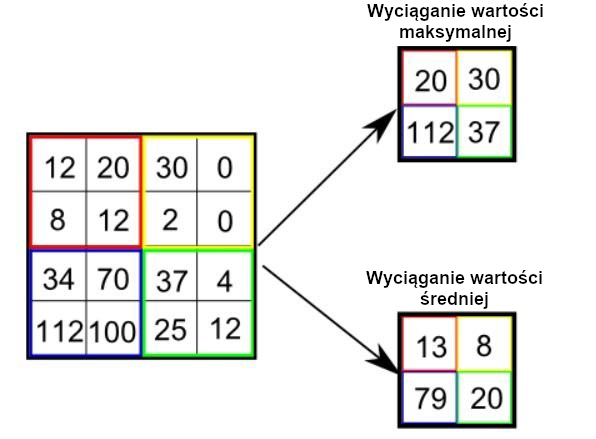
\includegraphics[width=5in]{pooling}
   \caption[Przykładowe operacje warstwy poolingu - źródło: Rysunek własny]{Przykładowe operacje warstwy poolingu}
   \label{fig:pooling}
  \end{figure}

  W modelu końcowym warstwy poolingu nie zostały zastosowane, aby uniknąć utraty
  kluczowych informacji przestrzennych koniecznych to właściwego wygenerowanie
  możliwych barw obrazu.

\subsubsection{Wykorzystywany zbiór treningowy}

  Do uczenia modelu został wykorzystany zbiór danych CIFAR-10 stworzony przez
  A. Krizhevsky oraz zaprezentowany w 2009 roku \cite{cifar-10}.
  Składa się on z 60000 obrazów w przestrzeni kolorów RGB o rozdzielczości 32 x 32 piksele.
  Spośród tych obrazów 10000 z nich zostało wykorzystanych jako zbiór
  walidacyjny do śledzenia skuteczności treningu modelu. Przykładowe obrazy
  ze zbioru danych zostały przedstawione na Rysunku \ref{fig:cifar10}.

  \begin{figure}[h]
   \centering
   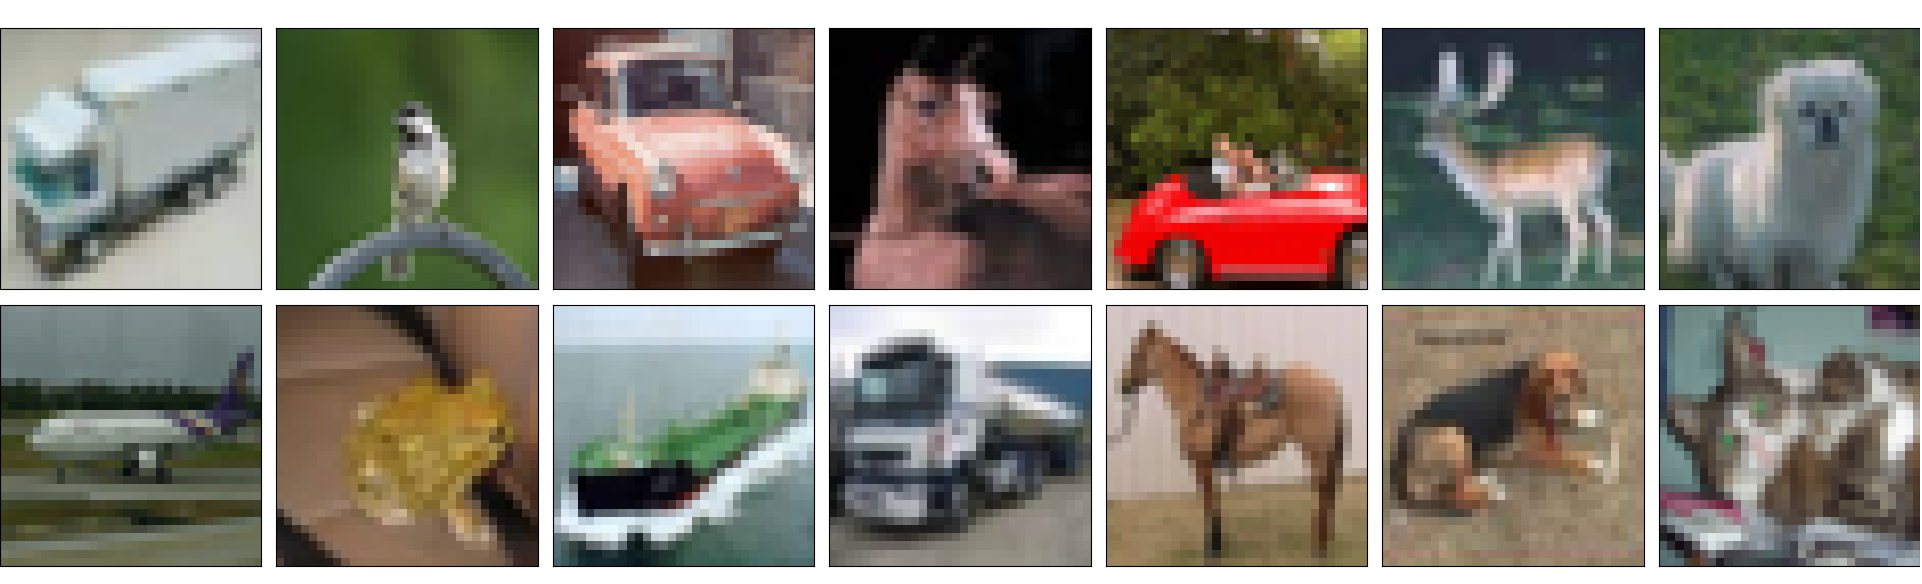
\includegraphics[width=5.5in]{cifar10}
   \caption[Przykładowe obrazy z CIFAR-10 - źródło: Rysunek własny]
   {Przykładowe obrazy z CIFAR-10}
   \label{fig:cifar10}
  \end{figure}

  Zaletą CIFAR-10 jest niewielka rozdzielczość obrazów co pozwala na mniej
  złożony model oraz szybszy proces uczenia, który można skutecznie przeprowadzić
  nawet przy ograniczonych możliwościach obliczeniowych. Ponadto zbiór ten składa
  się z obrazów dzielących się na 10 klas, tak mała różnorodność klas, a co za
  tym idzie, stosunkowo niewielka ilość możliwych obiektów pojawiających się
  na zdjęciach powinna ułatwić sieci wyuczenie się właściwych barw dla
  identyfikowanych powierzchni. Z drugiej strony mała ilość klas może niekorzystnie
  wpłynąć na umiejętność generalizacji modelu, jednakże obrazy z CIFAR-10
  przedstawiają zróżnicowane otoczenia zawierające obiekty nie kwalifikujące
  się do żadnej klasy, co powinno umożliwić wyuczenia się generalizacji przez
  sieć.

\subsubsection{Przetwarzanie wstępne danych} \label{Przetwarzanie wstępne danych}

  Przed podaniem na wejście sieci obrazy uczące były wpierw poddawane
  przetwarzaniu wstępnemu mającemu na celu doprowadzić do szybszego oraz
  stabilniejszego treningu modelu. Przetwarzanie wstępne jest kluczowe, gdyż
  wartości o jakie aktualizowane są wagi neuronu zależą w dużej mierze od
  wartości wejść tego neuronu. W przypadku gdy przedziały wartości tych wejść
  nie są jednolite, to może wystąpić duża różnica w tempie aktualizacji wag
  sieci, niektóre wagi będą zmieniane o wiele szybciej niż inne co może spowodować
  destabilizację treningu. Przeskalowanie wszystkich wartości wejściowych do jednakowych
  przedziałów, o niewielkiej wartości maksymalnej i minimalnej oraz wartości
  średniej zbliżonej do zera zmniejsza możliwość wystąpienia tego problemu
  oraz sprzyja ujednoliceniu tempa uczenia się przez sieć rozpoznawania różnych cech.
  Ponadto brak przeskalowania wejść może doprowadzić do zjawisk wybuchającego
  oraz zanikającego gradientu.

  % Przeskalowanie wszystkich wartości wejściowych do jednakowych
  % przedziałów, o niewielkiej wartości maksymalnej i minimalnej oraz wartości
  % średniej zbliżonej do zera, sprzyja ujednoliceniu tempa uczenia się przez sieć
  % rozpoznawania różnych cech.
  \noindent
  W ramach badania rozwiązania przetestowane zostały różne metody przetwarzania
  wstępnego zarówno danych wejściowych jak i pożądanej odpowiedzi:
  \begin{itemize}
  \item Normalizacja danych na przestrzeni całego zbioru danych z użyciem wartości
  maksymalnej oraz minimalnej całego zbioru, tak aby wartości pikseli danej składowej
  dla każdego obrazu zawierały się w przedziale od -0.5 do 0.5.
  \item Standaryzacja danych na przestrzeni całego zbioru danych z użyciem wartości
  średniej oraz odchylenia standardowego całego zbioru, tak aby uzyskać wartość
  średnią równą w przybliżeniu zero oraz jednostkowe odchylenie standardowe.
  \item Zastosowanie rozmycia gaussowskiego(ang. Gaussian blur) o różnej
  wielkości filtru Gaussowskiego.
  % \item Przepuszczenie składowej przez filtr Gaussa o różnej wielkości filtru.
  \end{itemize}

  Rozmycie gaussowskie, zwane także wygładzaniem gaussowskim (ang. Gaussian smoothing),
  jest to operacja polegająca na modyfikacji obrazu z użyciem filtru Gaussa.
  Stosuje się je w celu rozmycia detali na przetwarzanym obrazie, a także by
  ograniczyć ilość występujących na nim zakłóceń oraz szumów. Jest ono powszechnie
  stosowane w fazie przetwarzania wstępnego danych graficznych. W praktyce
  operacja ta sprowadza się do dokonywania splotu kolejnych fragmentów obrazu
  z funkcją Gaussa. Zastosowanie jej na danych wejściowych miało na celu
  zmniejszenie znaczenie detali na obrazie oraz ułatwienie sieci nauczenia się
  rozróżniania rozmaitych powierzchni oraz wzorców.

  Wymienione metody przetwarzania były stosowane w różnych połączeniach oraz
  konfiguracjach zarówno na składowej \textit{L}, jak i składowych \textit{A}
  oraz \textit{B}, a uzyskane wyniki opisane zostały w punkcie \ref{Rezultaty}

\subsubsection{Przetwarzanie końcowe danych}  \label{Przetwarzanie końcowe danych}

  Jeśli w trakcie procesu uczenia były stosowane zabiegi przetwarzania
  wstępnego danych wejściowych to podczas testowania modelu dane testowe również
  muszą być przetworzone w ten sam sposób, aby zapewnić poprawną pracę sieci.
  To samo dotyczy się danych wyjściowych sieci, jeśli podczas treningu z nadzorem
  pożądane wyjście było w pewien sposób przetworzone wstępnie to sieć uczy się
  odtwarzać te wyjście tak samo przetworzone, aby uzyskać oczekiwany efekty
  końcowy należy dokonać operacji odwrotnych do tych zastosowanych w fazie
  przetwarzania wstępnego. Przykładowo jeśli pożądana odpowiedź w procesie
  uczenia była normalizowana to podczas testów sieci jej wyście należy
  zdenormalizować, aby uzyskać oczekiwany rezultat. Jednakże my dla rozważanej
  problematyki proponujemy metodę alternatywną.

  Polega ona na uwydatnianiu kolorów wygenerowanych przez sieć dla wysokich
  wartości naświetlenia - składowej \textit{L}. Może być ona stosowana
  niezależnie od metody przetwarzania wstępnego danych wejściowych. Algorytm
  polega na przeskalowaniu pikseli składowych \textit{A} i \textit{B} tak, aby
  ich wartości mogły pokryć cały dostępny przedział wartości, ale dla danego
  piksela jego przedział jest ograniczony proporcjonalnie do stosunku wartości
  tego piksela w składowej \textit{L} do maksymalnej możliwej wartości pikseli
  składowej \textit{L}.

  Dla przykładu załóżmy, że wartość danego pikselu dla składowej \textit{A}
  wynosi 70, dla składowej \textit{B} wynosi -20, a dla składowej \textit{L} 80.
  Przedział wartości składowych \textit{A} i \textit{B} jest od -127 do 128, a
  składowej \textit{L} od 0 do 100. W następnym kroku znajdowana jest maksymalna
  absolutna wartość składowych \textit{A} i \textit{B} dla aktualnego obrazu.
  Załóżmy, że dla \textit{A} wynosi ona 90, a dla \textit{B} 60.
  Następnie piksele składowych \textit{A} i \textit{B} są dzielone przez
  swoje maksymalne wartości, a następnie rozciągnięte na cały dostępny przedział
  przez pomnożenie przez odpowiedni czynnik, czynnik ten jest z przedziału
  od 0 do 127 i jest wprost proporcjonalny do stosunku aktualnego piksela
  składowej \textit{L} do maksymalnej wartości \textit{L}, oznacza to, że jeśli
  dany piksel \textit{L} jest równy 100 to czynnik jest równy 127, a jeśli
  dany piksel \textit{L} jest równy 50 to wartość czynnika znajduje się w
  połowie swojego przedziału i równy jest 63,5.

  \noindent
  Dla podanych założeń otrzymujemy następujące nowe wartości piksela składowej \textit{A}
  ($p_{n}^{A}$) i piksela składowej \textit{B} ($p_{n}^{B}$):
  \begin{equation}
  p_{n}^{A} = \frac{70}{90} * 127 * \frac{80}{100} = 79.02
  \end{equation}
  \begin{equation}
  p_{n}^{B} = \frac{-20}{60} * 127 * \frac{80}{100} = -33.87
  \end{equation}

  \noindent
  Algorytm konwertowanie pikseli danej składowej można przedstawić wzorem:
  \begin{equation}
  S_{i, j}^{n} = \frac{S_{i, j}^{p}}{max\{abs\{S\}\}} * 127 * \frac{L_{i, j}}{100}
  \end{equation}

  \noindent
  Gdzie:
  \begin{itemize}
    \item $S$ - Konwertowana składowa będąca dwuwymiarowa macierzą pikseli.
    \item $S_{i, j}^{n}$ - Nowa wartość piksela (i, j) dla danej składowej.
    \item $S_{i, j}^{p}$ - Stara wartość piksela (i, j) dla danej składowej.
    \item $L_{i, j}$ - Wartość piksela (i, j) składowej jasności.
  \end{itemize}

  Zastosowanie powyższego algorytmu pozwoliło uzyskać bardziej zadawalające
  rezultaty działania modelu poprzez faworyzowanie kolorów tworzonych przez sieć
  dla powierzchni o dużej wartości jasności, jako, że wysoka jasność oferuje
  bardziej intensywne barwy. Kolorystyka powierzchni ciemnych pozostaje
  przytłumiona, jako, że brak naświetlenia ogranicza natężenie kolorów.

\subsubsection{Augmentacja danych}

  W celu skutecznego treningu modelu potrzebny jest odpowiednio duży i różnorodny
  zbiór treningowy. W obliczu problemu niewystarczającej ilości danych stosuje
  się metody zwane augmentacją danych pozwalające poszerzyć zbiór obrazów uczących
  poprzez dodawanie nowych informacji do obrazów będących podstawą zbioru tworząc
  w ten sposób nowe obrazy, które mogą być wykorzystane w treningu. Augmentacja
  danych przeciwdziała uczeniu się przez sieć nieistotnych wzorów i cech takich jak
  orientacja obiektu, jego umiejscowienie albo rozmiar. Dzięki temu model jest
  w stanie dogłębniej analizować obrazy wejściowe ucząc się rozpoznawać cechy
  o coraz to większym poziomie abstrakcji co przekłada się na o wiele lepiej
  rozwiniętą zdolność modelu do generalizacji danej problematyki.

  \noindent
  Do augmentacji stosuje się proste przekształcenia obrazu takie jak:
  \begin{itemize}
  \item Rotacja obrazu o wybrany kąt.
  \item Odbicie obrazu względem osi pionowej.
  \item Obcinanie skrajnych fragmentów obrazów (ang. crop).
  \item Zmiana odcienia oraz saturacji barw obrazu.
  \item Przybliżanie albo oddalanie treści obrazu.
  \item Modyfikacja rozdzielczości obrazu poprzez jego rozciąganie lub ściskanie.
  \item Tworzenie niewielkich ubytków w obrazach w losowych miejscach (ang. coarse dropout).
  \end{itemize}

  Należy jednak pamiętać, że nie wszystkie metody augmentacji nadają się do każdego zbioru
  danych, kluczowe jest, aby wybrać takie operacje, które poszerzają zbiór
  uczący o dane niosące znaczące oraz sensowne informacje patrząc z punktu wybranej
  problematyki oraz nie przesłaniają wzorców kluczowych do wyuczenia przez sieć.
  W przypadku zagadnienia kolorowania czarno-białych obrazów kluczową informacją
  jest kolor analizowanej powierzchni oraz jej cechy charakterystyczne, z tego
  powodu, do treningu modelu podstawowego nie zostały wykorzystane żadne metody
  augmentacji wpływające na barwy albo jasność obrazów. Wykluczone zostały również takie
  metody jak tworzeniu ubytków w obrazach, gdyż powoduje to niepotrzebną utratę
  informacji.
  W związku z tym, że wykorzystany zbiór CIFAR-10 posiada dużą ilość obrazów
  to w procesie uczenia została wykorzystana jedynie augmentacja poprzez
  odbicie obrazu względem osi pionowej z prawdopodobieństwem równym 50\%.

  % W zagadnieniu kolorowania czarno-białych obrazów informacjami najważniejszymi
  % są wartości pikseli powiązane z daną powierzchnią oraz cechy charakterystyczne
  % tych powierzchni, z tego powodu, aby ograniczyć straty
  % w procesie uczenia nie zastosowano żadnej
  % metody związanej ze zmianą barw obrazu wejściowego, jednocześnie nie można
  % było sobie pozwolić

\subsubsection{Funkcje kosztów} \label{Funkcje kosztów}
  % Bez teorii
  Kluczem do właściwego funkcjonowania modelu jest wybór odpowiedniej funkcji
  kosztu. W przypadku problematyki kolorowania czarno-białych obrazów ważne
  jest, aby wybrana funkcja kosztu uwzględniała specyficzną naturę problemu,
  gdzie dla niektórych przypadków właściwych jest wiele odpowiedzi. Jako
  przykład można podać taki obiekt jak samochód, który może być zarówno
  zielony, czerwony jak i żółty, każdy z tych kolorów powinien być oceniony
  jako właściwy, a wartość błędu wyliczona z użyciem funkcji kosztu dla tak
  wybranych przez sieć kolorów powinna odpowiednio to wskazywać. W ramach
  poszukiwań najbardziej odpowiedniej funkcji kosztu przetestowane zostały
  następujące funkcje.

  \begin{enumerate}[leftmargin=*]
  \item MSELoss (ang. Mean Squared Error Loss) - koszt oparty na błędzie średniokwadratowym
  przedstawiony funkcją:
  \begin{equation}
  Koszt = \frac{1}{n}\sum_{i=0}^{n} (x_{i} - y_{i})^2
  \end{equation}

  % \noindent
  % gdzie $x$ są to składowe \textit{A} oraz \textit{B} przewidziane przez sieć,
  % a $y$ to rzeczywiste \textit{A} i \textit{B}.

  \noindent
  Po dopasowaniu równania MSELoss do rozważanej problematyki otrzyma się:
  \begin{equation}
  Koszt = \frac{1}{n}\frac{1}{m}\sum_{i=0}^{n}\sum_{j=0}^{m} ((A_{i, j}^{P} - A_{i, j}^{R})^2 + (B_{i, j}^{P} - B_{i, j}^{R}))^2
  \end{equation}

  % \noindent
  % gdzie $(A_{i, j}^{R}$ i $(B_{i, j}^{R}$ są to rzeczywiste wartości składowych
  % \textit{A} i \textit{B} dla pikselu obrazy o współrzędnych $(i, j)$, a
  % $(A_{i, j}^{P}$ i $(B_{i, j}^{P}$ są to wartości przewidziane przez sieć.

  \item L1Loss zwany także MAELoss (ang. Mean Absolute Error Loss) - koszt oparty na
  średnim błędzie bezwzględnym dany funkcją:
  \begin{equation}
  Koszt = \frac{1}{n}\sum_{i=0}^{n} |x_{i} - y_{i}|
  \end{equation}
  % gdzie $x$ są to składowe \textit{A} oraz \textit{B} przewidziane przez sieć,
  % a $y$ to rzeczywiste \textit{A} i \textit{B}.

  \noindent
  Równanie L1Loss dla rozważanego zagadnienia:
  \begin{equation}
  Koszt = \frac{1}{n}\frac{1}{m}\sum_{i=0}^{n}\sum_{j=0}^{m} (|A_{i, j}^{P} - A_{i, j}^{R}| + |B_{i, j}^{P} - B_{i, j}^{R}|)
  \end{equation}
  % gdzie $x$ są to składowe \textit{A} oraz \textit{B} przewidziane przez sieć,
  % a $y$ to rzeczywiste \textit{A} i \textit{B}.

  \item SmoothL1Loss - zwany także \textit{Huber loss}, odmiana L1Loss przedstawiona w
  2015 roku przez R. Girshick \cite{SmoothL1Loss}. Jej zaletami są mniejsza
  czułość na elementy odstające (ang. outliner) i zmniejszona szansa na wystąpienie
  zjawiska eksplodującego gradientu.
  SmoothL1Loss przedstawiony jest funkcją:
  \begin{equation}
  Koszt = \frac{1}{n}\sum_{i=0}^{n} z_{i}
  \end{equation}

  \noindent
  gdzie $z_{i}$ dane jest:
  \begin{equation}
  z_{i} = \begin{cases}
               0.5(x_{i} - y_{i})^2 \text{, jeśli } |x_{i} - y_{i}| < 1 \\
               |x_{i} - y_{i}| - 0.5 \text{, w pozostałych przypadkach}
            \end{cases}
  \end{equation}

  \noindent
  Zastosowanie SmoothL1Loss do modelu podstawowego da następującą funkcję:
  \begin{equation}
  Koszt = \frac{1}{n}\sum_{i=0}^{n} (z_{i} + k_{i})
  \end{equation}

  \noindent
  gdzie $z_{i}$ dane jest:
  \begin{equation}
  z_{i} = \begin{cases}
               0.5(A_{i, j}^{P} - A_{i, j}^{R})^2 \text{, jeśli } |A_{i, j}^{P} - A_{i, j}^{R}| < 1 \\
               |A_{i, j}^{P} - A_{i, j}^{R}| - 0.5 \text{, w pozostałych przypadkach}
            \end{cases}
  \end{equation}

  \noindent
  a $k_{i}$ dane jest:
  \begin{equation}
  z_{i} = \begin{cases}
               0.5(B_{i, j}^{P} - B_{i, j}^{R})^2 \text{, jeśli } |B_{i, j}^{P} - B_{i, j}^{R}| < 1 \\
               |B_{i, j}^{P} - B_{i, j}^{R}| - 0.5 \text{, w pozostałych przypadkach}
            \end{cases}
  \end{equation}

  \end{enumerate}
  \noindent
  Gdzie:
  \begin{itemize}
    \item $x$ są to składowe \textit{A} oraz \textit{B} przewidziane przez sieć.
    \item $y$ to rzeczywiste składowe \textit{A} i \textit{B}.
    \item $A_{i, j}^{R}$ i $B_{i, j}^{R}$ są to rzeczywiste wartości składowych
    \textit{A} i \textit{B} dla pikselu obrazy o współrzędnych $(i, j)$.
    \item $A_{i, j}^{P}$ i $B_{i, j}^{P}$ są to wartości składowych
    \textit{A} i \textit{B} przewidziane przez sieć dla pikselu obrazy o
    współrzędnych $(i, j)$.
  \end{itemize}

  \noindent
  Szczegółowy opis skutków zastosowanie poszczególnych funkcji kosztów umieszczony
  został w punkcie \ref{Rezultaty}.

\subsubsection{Funkcje aktywacji}
  % ReLU
  W wyborze odpowiednej funkcji aktywacji kierowaliśmy się badaniami przeprowadzonymi
  przez B. Xu oraz jego współpracowników \cite{evaluatiuon_of_relu}. Testowali
  oni skuteczność takich funkcji jak ReLU, Leaky ReLU (pol. przepuszczające ReLU),
  PReLU (ang. Parametric ReLU) oraz RReLU (ang. Randomized Leaky ReLU) w
  zagadnieniu klasyfikacji treści obrazów. Bazując na otrzymanych przez nich
  rezultatach zdecydowaliśmy się wykorzystać w rozważanej problematyce funkcję
  aktywacji ReLU, przedstawioną na Rysunku \ref{fig:relu}

  \begin{figure}[h]
   \centering
   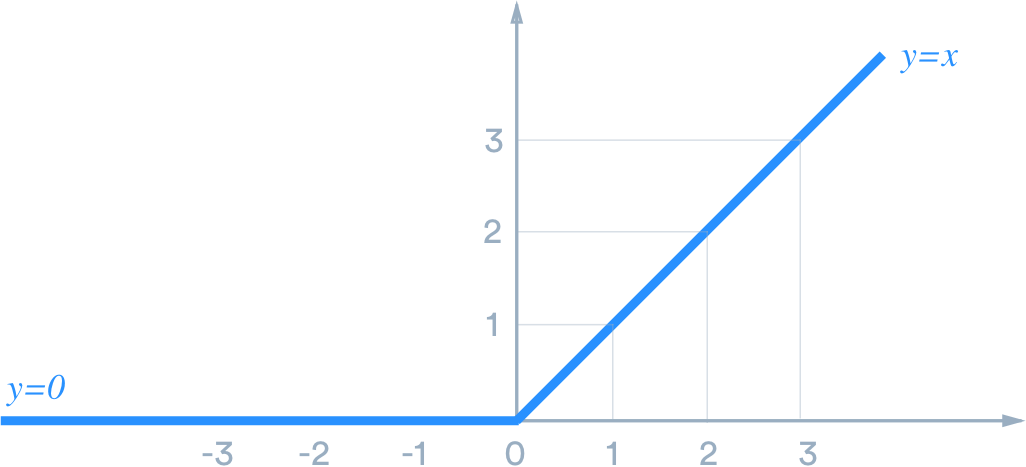
\includegraphics[width=4in]{relu}
   \caption[Funkcja aktywacji ReLU - źródło: \url{https://pytorch.org/docs/stable/_images/ReLU.png}]
   {Funkcja aktywacji ReLU}
   \label{fig:relu}
  \end{figure}

  Funkcja ta posiada wiele zalet takich jak przyspieszenie procesu zbieganie się stanu
  sieci do stanu pożądanego poprzez brak ograniczeń na maksymalną wartość
  funkcji oraz niska złożoność obliczeniowa.
  Ponadto funkcja ta, w związku z zerową wartością dla ujemnych argumentów,
  zapewnia aktywację neuronów modelu tylko wtedy, gdy analizują one wzorce
  kluczowe dla nich samych oraz danego zagadnienia, zwiększa to odporność modelu na
  szumy wejściowe oraz przeuczanie, a także poprawia zdolności predykcyjne sieci.

  Jednakże stosowanie ReLU tworzy zagrożenie blokowanie się procesu uczenia,
  jeśli dojdzie do sytuacji, w której wagi modelu dojdą do stanu, gdzie wartość
  aktywacji będzie zbliżona do zera. Spowoduje to zerową wartość gradientu
  podczas fazy wstecznej propagacji błędu powodując wstrzymanie się procesu
  aktualizowania wag modelu, a w rezultacie, nieefektywny proces uczenia.
  Pomimo to jednak zostaliśmy przy wyborze funkcji ReLU wierząc, że pozostałe
  zabiegi takie jak zastosowanie warstw BatchNorm pozwolą zminimalizować
  niepożądane efekty tego zjawiska.

\subsubsection{Algorytmy optymalizacyjne} \label{Algorytmy optymalizacyjne}
  % Bez teorii
  % TODO: Może dać bardziej szczegółowy opis
  % TODO: Zacytować twórców Adam i Adagrad, linki do paperów są w dokumentacji
  % pytorcha o tych algorytmach
  Podczas planowanie treningu modelu należy zdecydować się na odpowiedni
  algorytm optymalizacyjny, właściwa decyzja pozwala uniknąć zatrzymania się
  procesu uczenia w lokalnych minimach co zwiększa końcową dokładność oraz
  skuteczność modelu.
  Podczas badań przetestowane zostały różne algorytmy optymalizacyjne,
  a uzyskane rezultaty zostały szczegółowo opisane oraz porównane w punkcie
  \ref{Rezultaty}.\newline
  Wykorzystane zostały następujące algorytmy:
  \begin{itemize}
    \item Adam (ang. Adaptive Moment Estimation)
    \item Adagrad (ang. Adaptive Gradient Algorithm)
    \item SGD (ang. Stochastic Gradient Descent)
  \end{itemize}

  \noindent
  Przeprowadzone zostały także poszukiwania najbardziej odpowiednich hiperparametrów
  dla wymienionych algorytmów w celu osiągnięcia jak największej ich skuteczności
  w rozwiązaniu rozważanej problematyki.

% TODO: Od tego momentu było ekspres pisanie, wiec może do zredagowania
\subsubsection{Trening}

Model trenowaliśmy paczkami o wielkości 128 obrazów, cała epoka składała się z
50000 obrazów. Przed każdą epoką zbiór treningowy był przetasowywany, aby
przeciwdziałać przeuczaniu się sieci. Aby znaleźć najbardziej zadowalające rozwiązanie
przetestowane zostały różne konfiguracje treningowe, możliwe zmienne elementy
konfiguracji to algorytmy optymalizacyjne opisane w punkcie
\ref{Algorytmy optymalizacyjne}, funkcje kosztów opisane w punkcie \ref{Funkcje kosztów},
rodzaje przetwarzania wstępnego opisane w punkcie \ref{Przetwarzanie wstępne danych} oraz
skutki zastosowanie takich warstw jak Dropout (punkt \ref{Dropout}) oraz BatchNorm
(punkt \ref{BatchNorm}). Jako funkcja aktywacji wybrana została funkcja ReLU.
Dla różnych konfiguracji została także przedstawiona charakterystyka porównawcza.


\subsubsection{Rezultaty} \label{Rezultaty}

 Uzyskane wyniki są w znacznej mierze zależne od wybranej konfiguracji.
 Najbardziej satysfakcjonujące rezultaty uzyskane przez model zostały
 przedstawione na Rysunku \ref{fig:best_result}

 \begin{figure}[ht]
   \centering
   \subfloat[Obraz spoza zbioru uczącego]{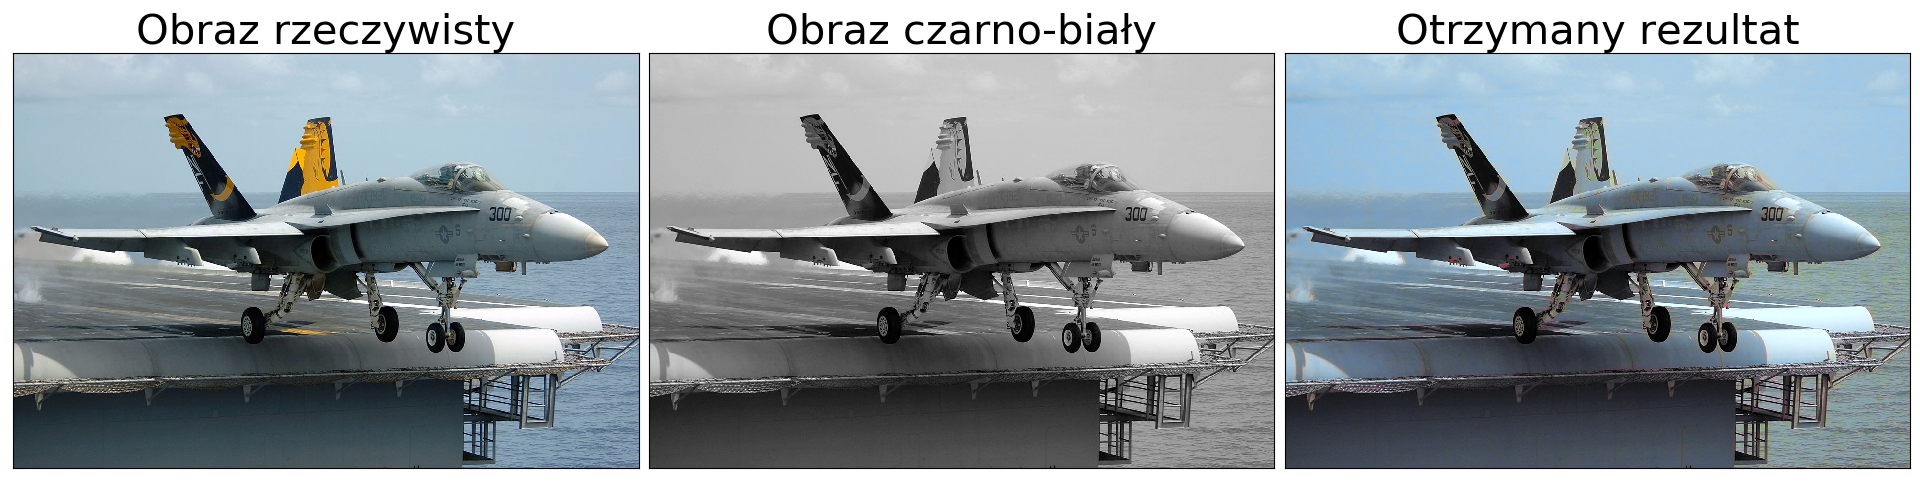
\includegraphics[width = 4.5in]{best_results_plane}} \\
   \subfloat[Obraz spoza zbioru uczącego]{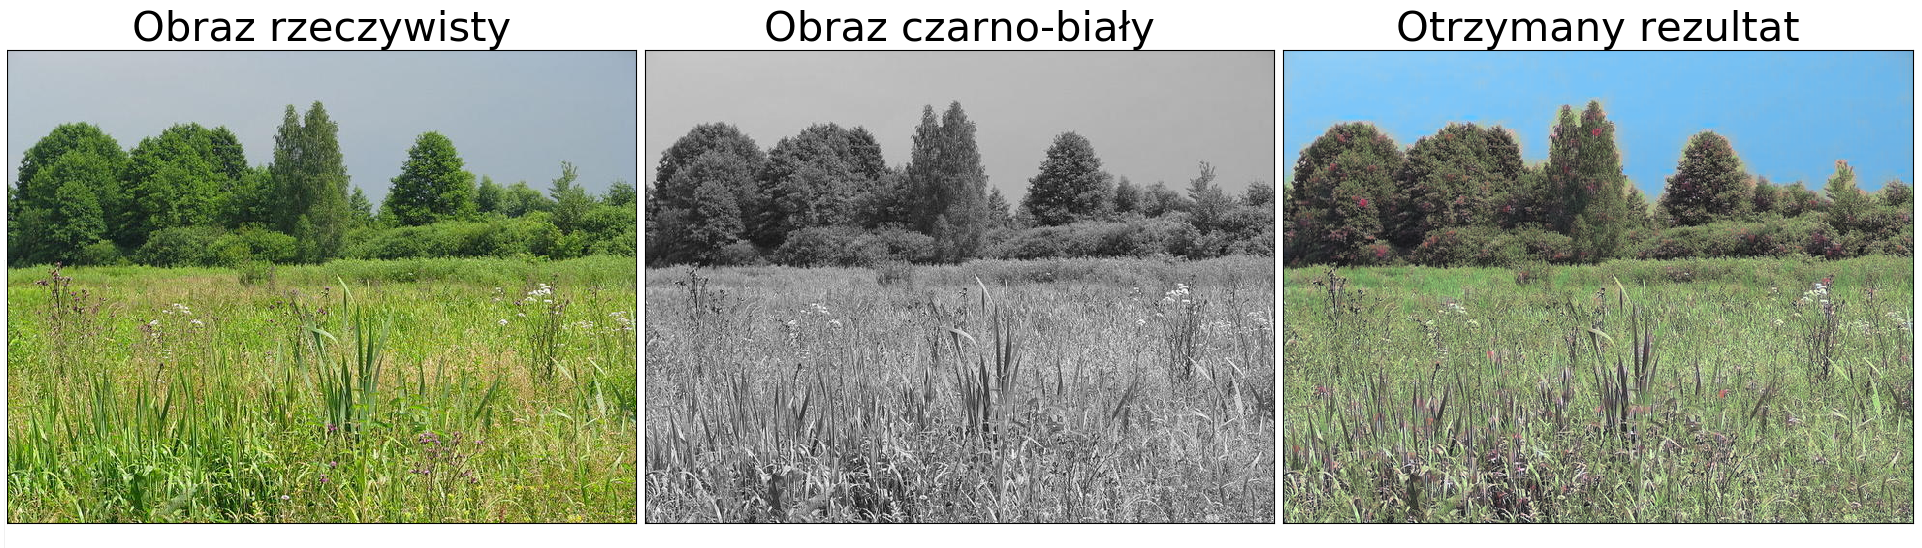
\includegraphics[width = 4.5in]{best_results_krajobraz}} \\
   \subfloat[Obraz ze zbioru uczącego]{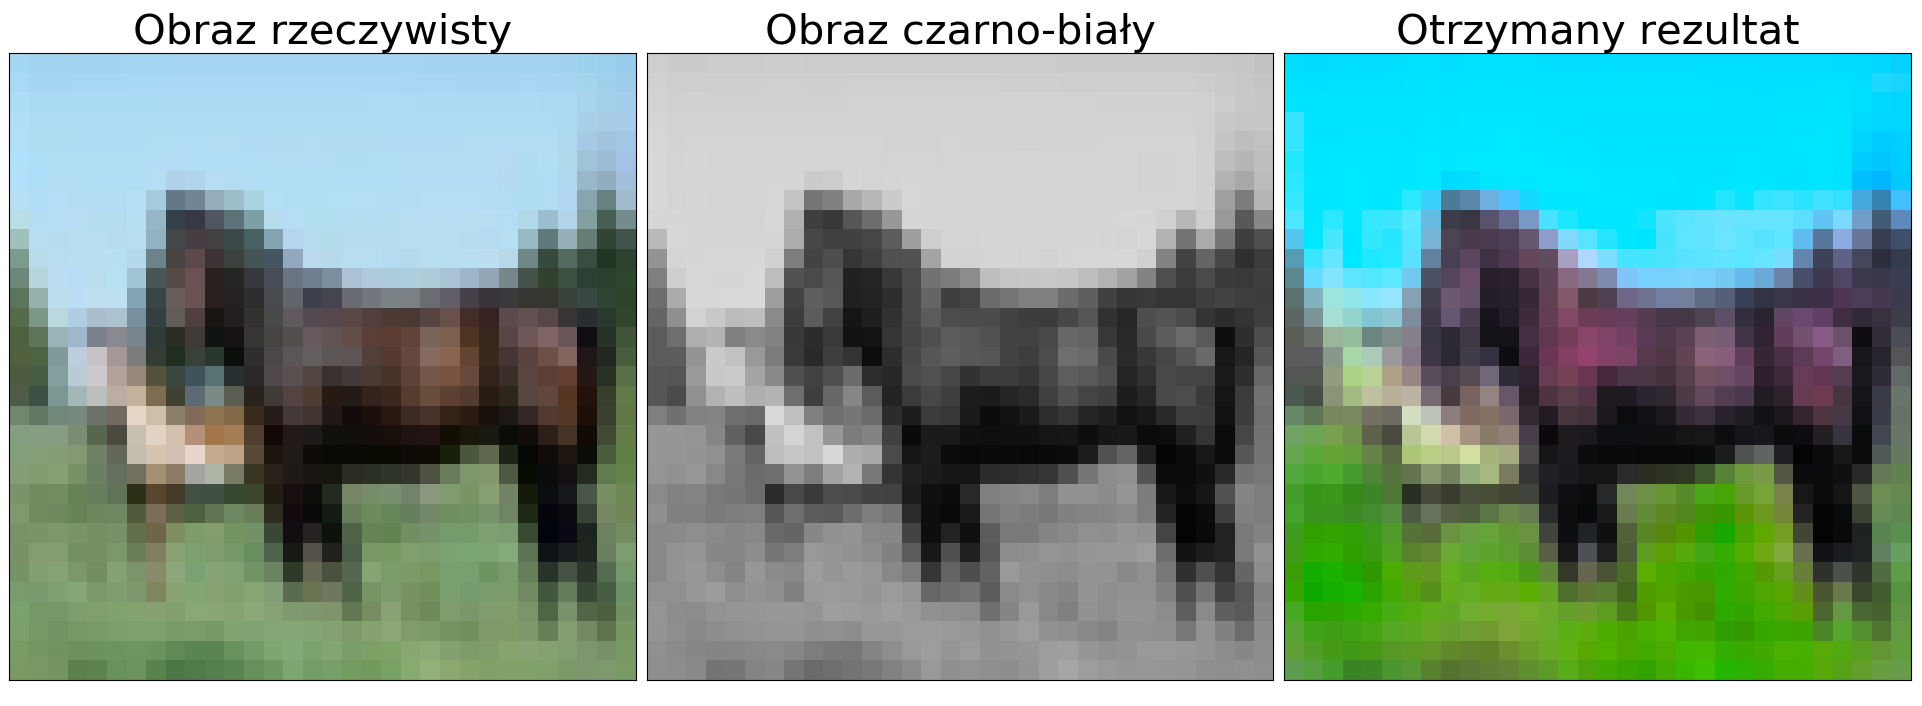
\includegraphics[width = 4.5in]{best_results_horse}} \\
   \caption[Efekty działania sieci - źródło: Rysunek własny bazujący na:
   \url{https://fr.m.wikipedia.org/wiki/Fichier:An_F-A-18C_Hornet_launches_from_the_flight_deck_of_the_conventionally_powered_aircraft_carrier.jpg},
   \url{https://pl.wikipedia.org/wiki/Plik:PL_Bagno_Calowanie_2.jpg}, \cite{cifar-10}]
   {Rezultaty.}
   \label{fig:best_result}
 \end{figure}

 \noindent
 Efekt ten został uzyskany przy następującej konfiguracji:
 \begin{itemize}
   \item Funkcja kosztu MSELoss.
   \item Funkcja aktywacji ReLU.
   \item Algorytm optymalizacyjny Adam.
   \item Normalizacja składowej \textit{L} podczas przetwarzania wstępnego.
   \item Standaryzacja składowych \textit{A} i \textit{B} podczas przetwarzania wstępnego.
   \item Nie zastosowanie rozmycia Gaussowskiego.
   \item Zastosowanie warstwy BatchNorm oraz nie zastosowanie warstwy Dropout.
   \item Zastosowanie zaproponowanego przez nas algorytmu przetwarzania końcowego.
 \end{itemize}

 \noindent
 Na podstawie obrazów na Rysunku \ref{fig:best_result} oraz przeprowadzonych
 testów można wywnioskować, że model nauczył się najlepiej kolorować powierzchnie
 o zazwyczaj stałej barwie takie jak niebo albo trawa, widać, że ich barwy są
 wyjątkowo intensywne oraz jednoznacznie wskazują co to są za powierzchnie.
 Gorzej rzecz się ma z obiektami o zmiennych barwach takimi jak na przykład
 samochody, w związku z ich zmienną barwą na przestrzeni całego zbioru danych
 model, chcąc zminimalizować błąd liczony przez funkcję kosztu, uśredniał kolor
 tych obiektów co skutkuje ich przytłumionymi barwami przechodzącymi często
 w odcienie brązu. Z tego powodu pomniejsze detale na kolorowanych zdjęciach
 tracą swoje barwy, efekty tego zjawiska można zaobserwować analizując
 stateczniki odrzutowca ukazanego na obrazie \textit{(a)} Rysunku \ref{fig:best_result}.
 Wykres uczenia przedstawionego modelu został przedstawiony na Rysunku
 \ref{fig:loss_plot}. Można zaobserwować stopniowy spadek wartości funkcji
 kosztu, co oznacza poprawne zbieganie się modelu do właściwego rozwiązania.
 W końcowych fazach wykresu widać, że wartość kary zmienia się o bardzo
 małe wartości, co znaczy, że proces uczenia wpadł już w minimum będące
 jednym z dostępnych rozwiązań.

 \begin{figure}[h]
  \centering
  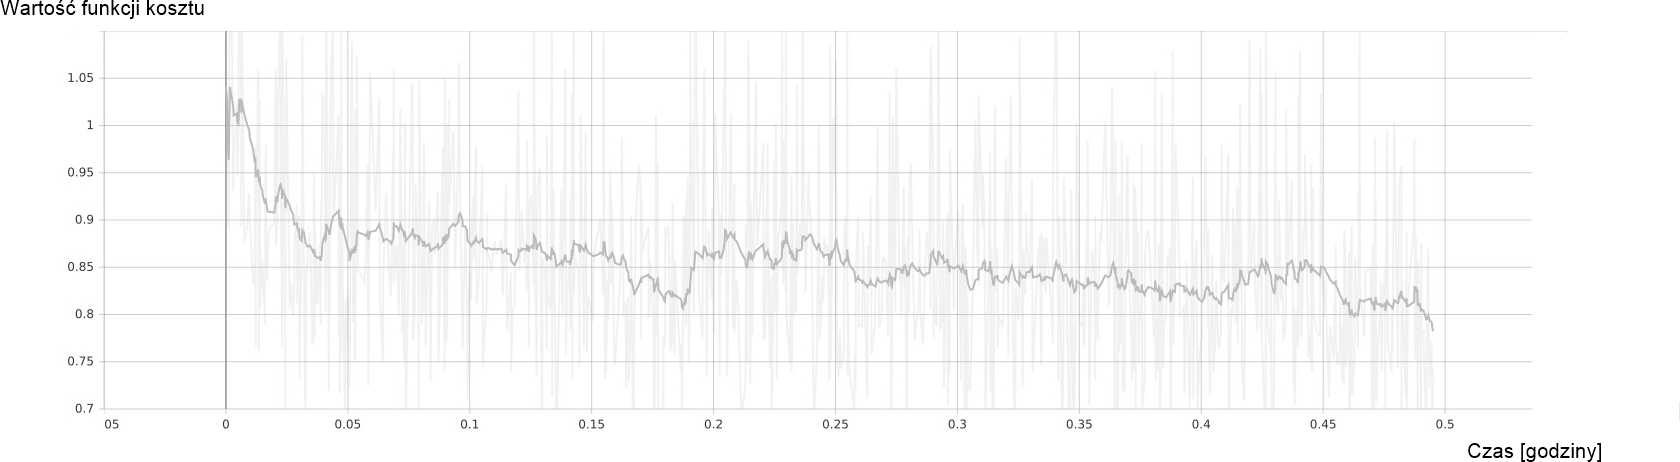
\includegraphics[width=6in]{loss_plot}
  \caption[Wykres uczenia modelu końcowego - źródło: Rysunek własny]
  {Wykres uczenia modelu końcowego}
  \label{fig:loss_plot}
 \end{figure}

  \noindent
  W dalszej części sekcji opisany został wpływ poszczególnych elementów konfiguracji.

  Największy wpływ na uzyskiwane rezultaty ma zastosowanie algorytmu przetwarzania
  końcowego opisanego w punkcie \ref{Przetwarzanie końcowe danych}. Pomógł on
  znacznie wzbogacić kolory generowane przez sieć. Odpowiednie porównanie
  zostało przedstawione na Rysunku \ref{fig:trick}. Wadami tej metody są generowane
  momentami zbyt intensywne barwy zdjęć oraz bardziej widoczne czasami
  zdarzające się "wycieki"
  kolorów jednych powierzchni na inne, przykładowo czerwony kolor z samochodu
  wychodzi poza powierzchnię samochodu i barwi fragmenty trawy przylegające do
  samochodu na czerwono. Efekt ten jest znacznie mniej widoczny przy zdjęciach
  o wysokiej rozdzielczości, co sprawia, że w zastosowaniu praktycznym ta
  wada modelu jest do zaakceptowania. Na Rysunku \ref{fig:trick} widać to
  poprzez drobne obszary żółci na granicy nieba i drzew.

  \begin{figure}[H]
   \centering
   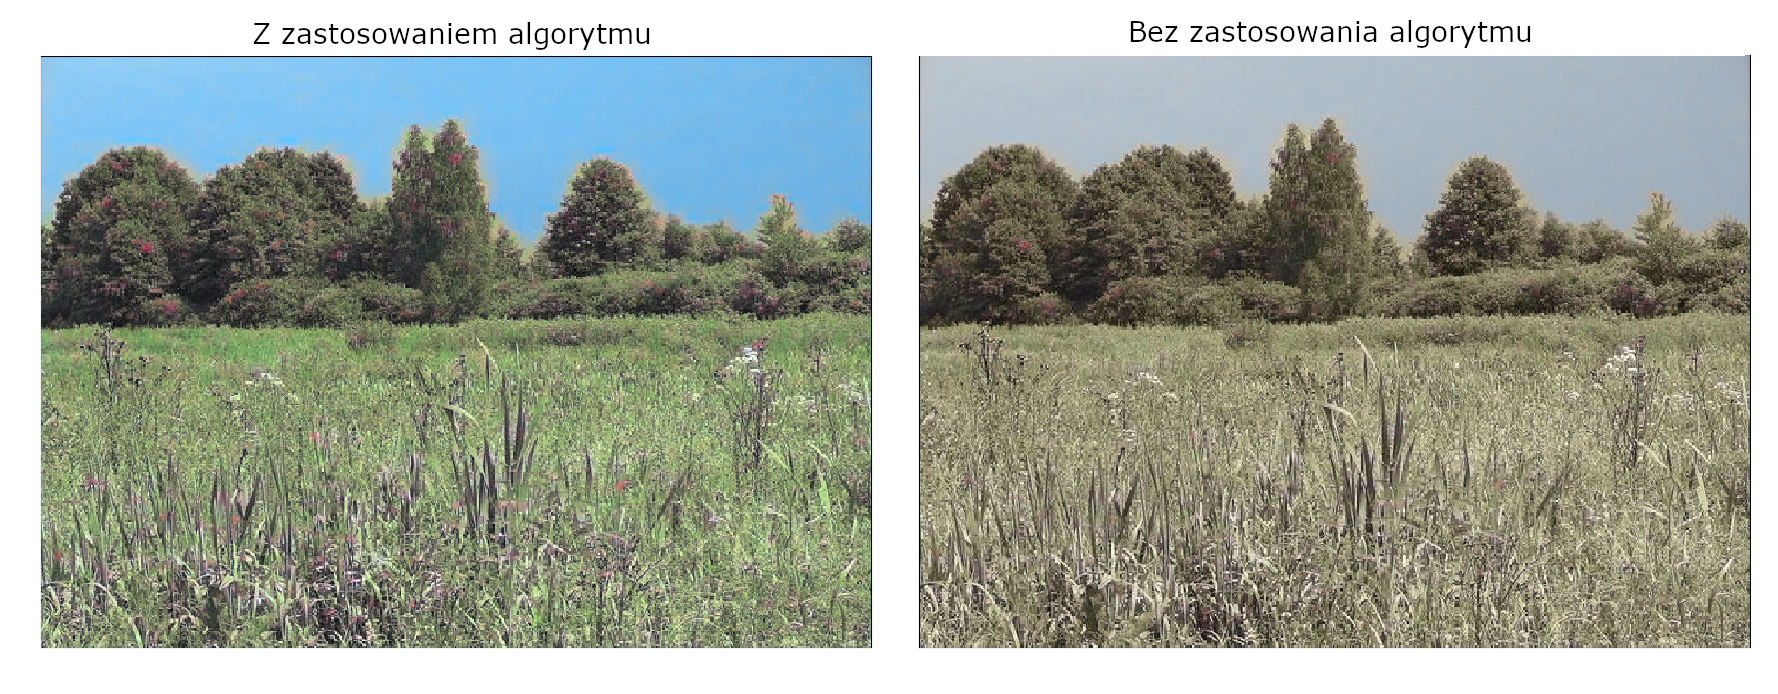
\includegraphics[width=6in]{porownania_trick_krajobraz}
   \caption[Efekt zastosowania algorytmu przetwarzania końcowego - źródło
   rysunek własny na podstawie: \url{https://pl.wikipedia.org/wiki/Plik:PL_Bagno_Calowanie_2.jpg}]
   {Efekt zastosowania algorytmu przetwarzania końcowego}
   \label{fig:trick}
  \end{figure}

  Kolejnym ważnym komponentem jest użyta funkcja kosztu, właściwy wybór
  znaczenie poprawia proces aktualizowania się wag sieci, co przekłada się
  na lepsze rezultaty. Kluczowe było, aby funkcja straty uwzględniała
  możliwą wielobarwność kolorowanych obiektów i nie karała sieci za barwy niezgodne
  z barwami na obrazie rzeczywistym, ale pasujące w kontekście kolorowanej
  powierzchni. Na Rysunku \ref{fig:porownanie_funkcji_kosztu} zostało
  umieszczone porównanie rezultatów modeli uczonych z użyciem różnych funkcji
  kosztu, przedstawione obrazy zostały wygenerowane bez użycia algorytmu
  końcowego przetwarzania w celu uwydatnienia cech funkcji kosztu.

  \begin{figure}[H]
   \centering
   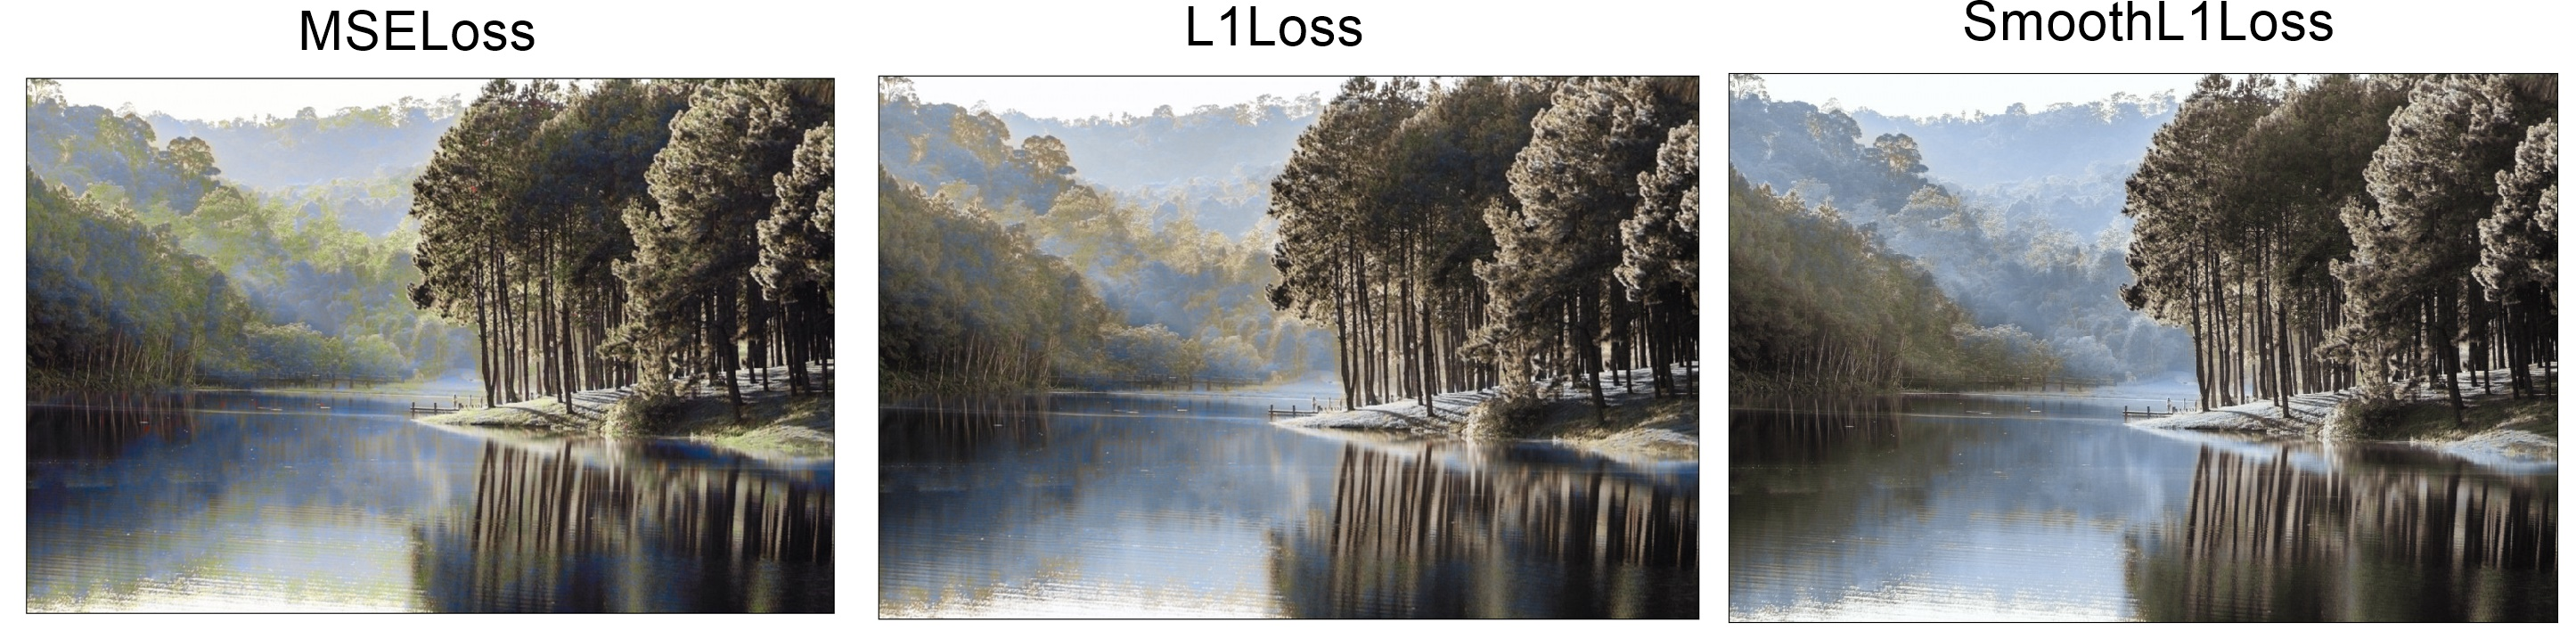
\includegraphics[width=6in]{porownanie_funkcji_kosztu}
   \caption[Porównanie rezultatów modeli uczonych z użyciem różnych funkcji
   kosztu - źródło rysunek własny na podstawie: \url{https://cdn.thearthunters.com/wp-content/uploads/2013/06/bg-960x636.jpg}]
   {Porównanie rezultatów modeli uczonych z użyciem różnych funkcji
   kosztu.}
   \label{fig:porownanie_funkcji_kosztu}
  \end{figure}

  \noindent
  L1Loss: Testując funkcję kosztu L1Loss oczekiwano, że uzyskiwane obrazy będą
  cechowały się niską saturacją, a generowane kolory będą przytłumione. Jest
  to spowodowane skłonnościami funkcji L1Loss do uśredniania wyjścia modelu w
  przypadku, kiedy kolorowana powierzchnia ma zmienną barwę na przestrzeni
  zbioru uczącego. Działanie L1Loss ma na celu zminimalizować błąd bezwzględny
  będący różnicą pomiędzy kolorami tych powierzchni, a kolorami generowanymi
  przez sieć, co skutkuje barwą o wartości znajdującej się pomiędzy wartościami
  wszystkich występujących kolorów dla powierzchni danego typu. W rezultacie
  otrzymywane są obrazy w kolorze sepii, co widać na Rysunku
  \ref{fig:porownanie_funkcji_kosztu}.

  \noindent
  SmoothL1Loss: Funkcja ta bazuje na L1Loss, ale tworzy kryterium, które przy
  błędzie bezwzględnym o wartości mniejszej niż 1 używa kwadratu z wartości
  błędu, a w pozostałych przypadkach używa wartości bezwzględnej błędu. Wzór
  L1Loss jest przedstawiony w punkcie \ref{Funkcje kosztów}. Zabieg ten sprawia,
  że funkcja jest mniej czuła na elementy odstające oraz przeciwdziała zjawisku
  eksplodującego gradientu. Funkcja to została zastosowana jako próba skuteczniejszego
  wyuczenia się przez model kolorów detali występujących na obrazach oraz aby przeciwdziałać
  uśrednianiu wartości barw przez sieć. Jednakże efekt ten nie został uzyskany,
  a przeciwdziałanie elementom odstającym przez SmoothL1Loss dodatkowo negatywnie wpłynęło na
  kolory generowane przez sieć. Funkcja wylicza mniejszy błąd, gdy
  wartość różnicy bezwzględnej pomiędzy wyjściem sieci, a kolorem
  rzeczywistym jest wysoka, co skutkuje tendencją modelu do
  generowania składowych \textit{A} i \textit{B} o wartościach ze środka
  przedziału wartości, czyli w okolicy zera. W praktyce jednak wartości tych
  składowych są ograniczane przez składową \textit{L} będącą jasnością obrazu,
  czego wynikiem są średnie wartości generowanych \textit{A} i \textit{B} lekko poniżej zera.
  Takie wartości odpowiadają głównie odcieniom niebieskiego i trochę odcieniom
  zielonego, co wyraźnie widać na Rysunku \ref{fig:porownanie_funkcji_kosztu}.

  \noindent
  MSELoss: W związku z brakiem algorytmu, który wstrzymuje karanie modelu w
  sytuacji, gdy generowane kolory są niezgodne z rzeczywistymi, ale prawdopodobne
  dla kolorowanej powierzchni to funkcja MSELoss również ma tendencję do
  uśredniania generowanych kolorów jak funkcja L1Loss. Jednakże większa czułość funkcji
  na wysokie wartości błędów, powodowana podnoszeniem różnicy pomiędzy wartością
  przewidzianą a rzeczywistą do kwadratu,
  umożliwiła wytrenowanie modelu zdolnego do generowania
  barw z szerokiego zakresu wartości, co korzystnie wpłynęło na rezultaty.
  Pokolorowany obraz wygenerowane przez model uczony z użyciem funkcji MSELoss prezentuje
  się najlepiej spośród obrazów na Rysunku \ref{fig:porownanie_funkcji_kosztu},
  z tego powodu oraz w związku z korzystnym efektem zastosowania MSELoss, właśnie
  ta funkcja została wybrana w procesie uczenia modelu końcowego.

  Wybór odpowiedniego algorytmu optymalizacyjnego może znacznie poprawić rezultaty
  modelu poprzez odpowiednie nakierowanie jego wag aby wartość kary wyliczana
  przez funkcję kosztu była jak najmniejsza. Minimalizowanie wartości tej kary
  jest zagadnieniem złożonym, w trakcie poszukiwania optimum dla wag sieci
  występują liczne minima lokalne, które utrudniają odnalezienie minimum '
  globalnego zapewniającego najbardziej satysfakcjonujące wyniki. Aby
  przeciwdziałać zatrzymaniu się procesu uczenia w lokalnych minimach należy
  zastosować odpowiedni algorytm optymalizacyjny. Przykładowy obraz pokolorowany
  przez model uczony z użyciem różnych algorytmów optymalizacyjnych został
  przedstawiony na Rysunku \ref{fig:porownanie_optimizerow}

  \noindent
  Dla algorytmu Adam zostały wybrane parametry: $\beta_{1} = 0.9$, $\beta_{2} = 0.999$,
  $\text{wskaźnik uczenia} = 0.1$, $\text{współczynnik zaniku wag} = 1e-10$ oraz
  $eps=1e-08$.
  \newline
  Dla algorytmu Adagrad zostały wybrane parametry: $\text{wskaźnik uczenia} = 0.1$,
  $\text{współczynnik zaniku wskaźnika uczenia} = 0.999$,
  $\text{współczynnik zaniku wag} = 1e-10$ oraz $eps=1e-10$.
  \newline
  Dla algorytmu SGD zostały wybrane parametry: $\text{wskaźnik uczenia} = 0.1$,
  $\text{pęd} = 0.9$, $\text{tłumienie} = 0$ oraz $\text{współczynnik zaniku wag} = 0$.
  Zmianę wskaźnika uczenia dla SGD nadzorował planista o parametrach:
  $\text{wielkość kroku} = 1$ oraz $\text{gamma} = 0.999$.

  \begin{figure}[H]
   \centering
   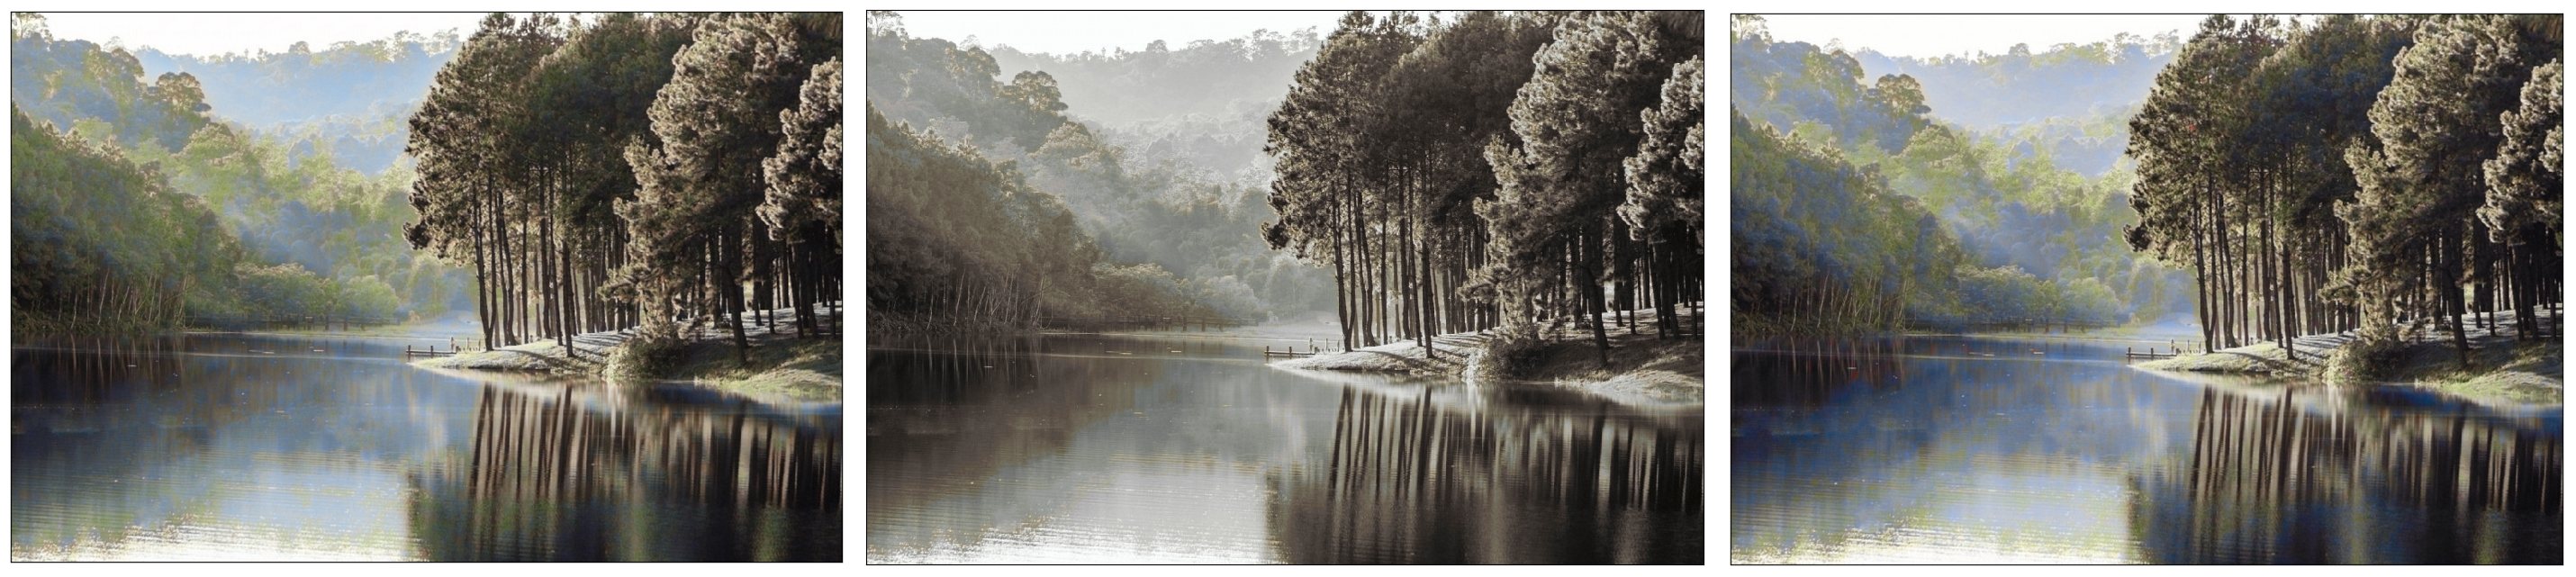
\includegraphics[width=6in]{porownanie_optimizerow}
   \caption[Porównanie rezultatów modeli uczonych z użyciem różnych algorytmów
   optymalizacyjnych - źródło rysunek własny na podstawie: \url{https://cdn.thearthunters.com/wp-content/uploads/2013/06/bg-960x636.jpg}]
   {Porównanie rezultatów modeli uczonych z użyciem różnych algorytmów
   optymalizacyjnych}
   \label{fig:porownanie_optimizerow}
  \end{figure}

  \noindent
  Jako algorytm optymalizacyjny dla modelu końcowego został wybrany Adam,
  decyzja ta jest oparta na wielu kryteriach takich jak wartości końcowe funkcji
  kosztu oraz wizualne efekty działania sieci. Przykładowa ocena wizualna
  została opisana bazując na Rysunku \ref{fig:porownanie_optimizerow}.
  Porównując pokolorowane obrazy można zauważyć, że najgorzej prezentuje się
  rezultat modelu stosujący algorytm Adagrad, na obrazie tym nie występuje wiele
  kolorów i dominują barwy szarości. Algorytm ten jest przeznaczony do
  pracy z rzadkimi zbiorami treningowymi, a zastosowany zbiór CIFAR-10 takim nie
  jest, można więc podejrzewać, że podczas procesu uczenia, wagi sieci na
  płaszczyźnie funkcji celu wpadły w minimum lokalne i nie były w stanie z niego
  wyjść, co poskutkowało pominięciem minimum globalnego będącego najlepszym
  możliwym rozwiązaniem. Analizując obrazy dla algorytmów Adam oraz SGD
  można zauważyć, że są one znacznie lepiej pokolorowane niż obraz dla
  algorytmu Adagrad. Można na nich wyraźnie wyróżnić roślinność pokolorowaną
  na zielono oraz taflę wody w odcieniach niebiskiego. Jednakże pomimo
  znacznego podobieństwa pomiędzy tymi dwoma obrazami można zauważyć, że tafla
  wody jest znacznie bardziej wypełniona kolorem na obrazie dla algorytmu Adam,
  co świadczy, że algorytm ten był w stanie zapewnić lepsze minimum dla wag
  sieci, co zapewniło modelowi lepiej rozwiniętą zdolność predykcji kolorów dla
  różnorodnych powierzchni.

  Z powodów opisanych w punkcie \ref{Dropout} warstwa Dropout nie została użyta
  w modelu końcowym. Na Rysunku \ref{fig:porownanie_dropout} został pokazany
  wpływ zastosowania tej warstwy w modelu na kolorowane przez model obrazy w zależności od
  wartości parametru \textit{p} (prawdopodobieństwo dezaktywowania dla każdego
  neuronu sieci).

  \noindent
  Jak widać zastosowanie tej warstwy nie przyniosło żadnych korzyści. Dla
  małych wartości parametru \textit{p} barwy na kolorowanym obrazie są
  mniej żywe niż bez zastosowania Dropout, a dla większych wartości widać, że
  model traci w dużej mierze swoje zdolności do predykcji kolorów. Dowodzi to,
  że w przypadku rozważanej problematyki większym zagrożeniem jest utrata
  kluczowych informacji o obrazie niż niebezpieczeństwo przeuczenia sieci, co
  sprawia, że warstwa Dropout staje się niepożądana.

  \begin{figure}[H]
   \centering
   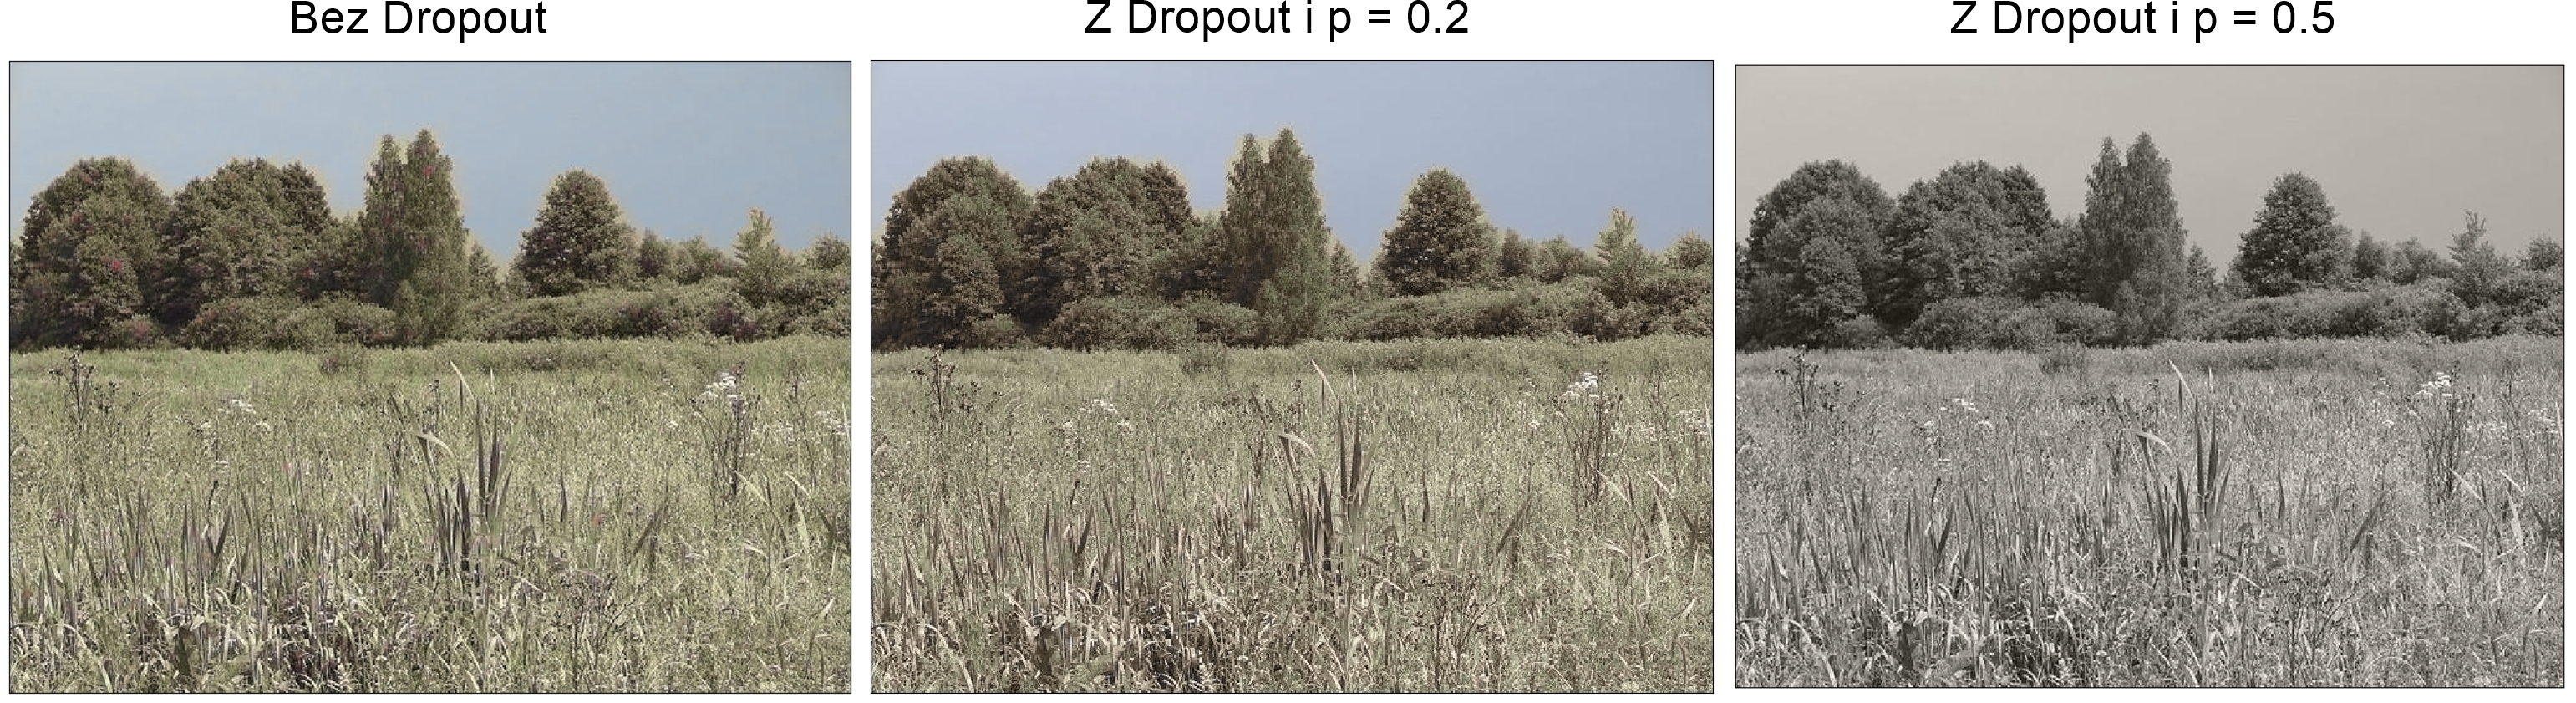
\includegraphics[width=6in]{porownanie_dropout}
   \caption[Wpływ zastosowania warstwy Dropout na kolorowanie obrazów - źródło: rysunek własny na podstawie:
   \url{https://pl.wikipedia.org/wiki/Plik:PL_Bagno_Calowanie_2.jpg}]
   {Wpływ zastosowania warstwy Dropout na kolorowanie obrazów}
   \label{fig:porownanie_dropout}
  \end{figure}

  Duże znaczenie dla jakości treningu modelu miał także wybór metod przetwarzania
  wstępnego zarówno obrazów wejściowych jak i obrazów referencyjnych. Przyczyny
  zastosowania takich zabiegów zostały dokładnie opisane w punkcie
  \ref{Przetwarzanie wstępne danych}.
  Porównanie efektów zastosowania różnych metod w różnych konfiguracjach zostało umieszczone
  na Rysunku \ref{fig:porownanie_preprocessing}, a dokładny opis konfiguracji
  został umieszczony w Tabeli \ref{table:preprocessing}.

  \begin{figure}[ht!]
    \centering
    \subfloat[]{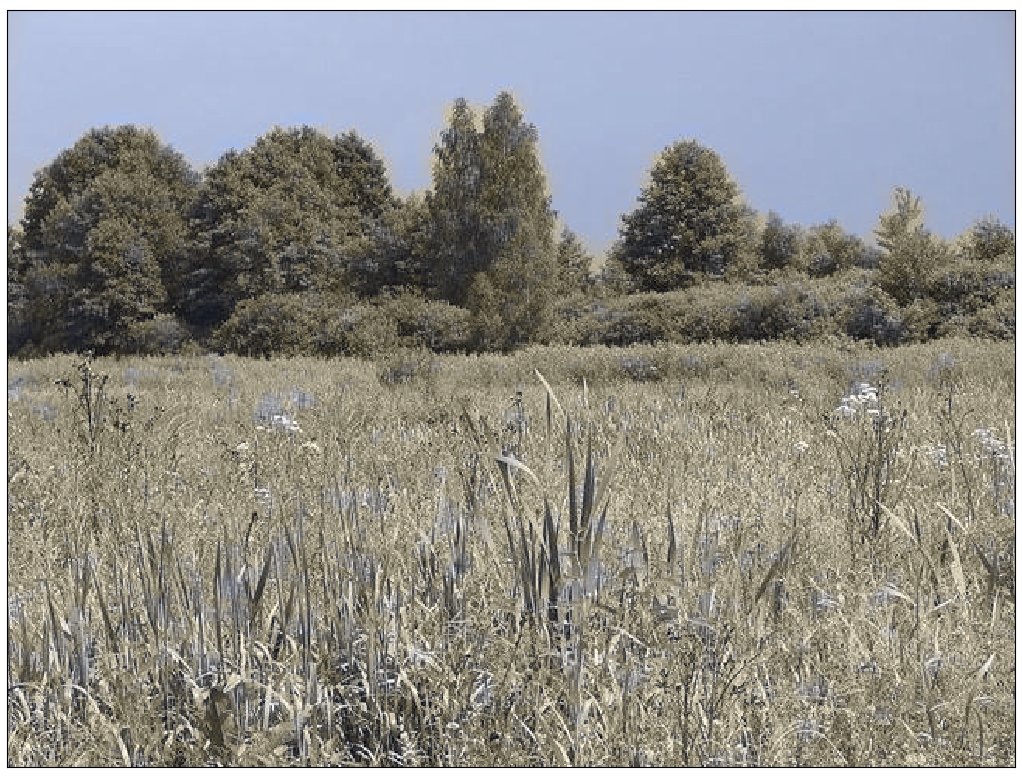
\includegraphics[width = 2in]{norm_norm}}
    \subfloat[]{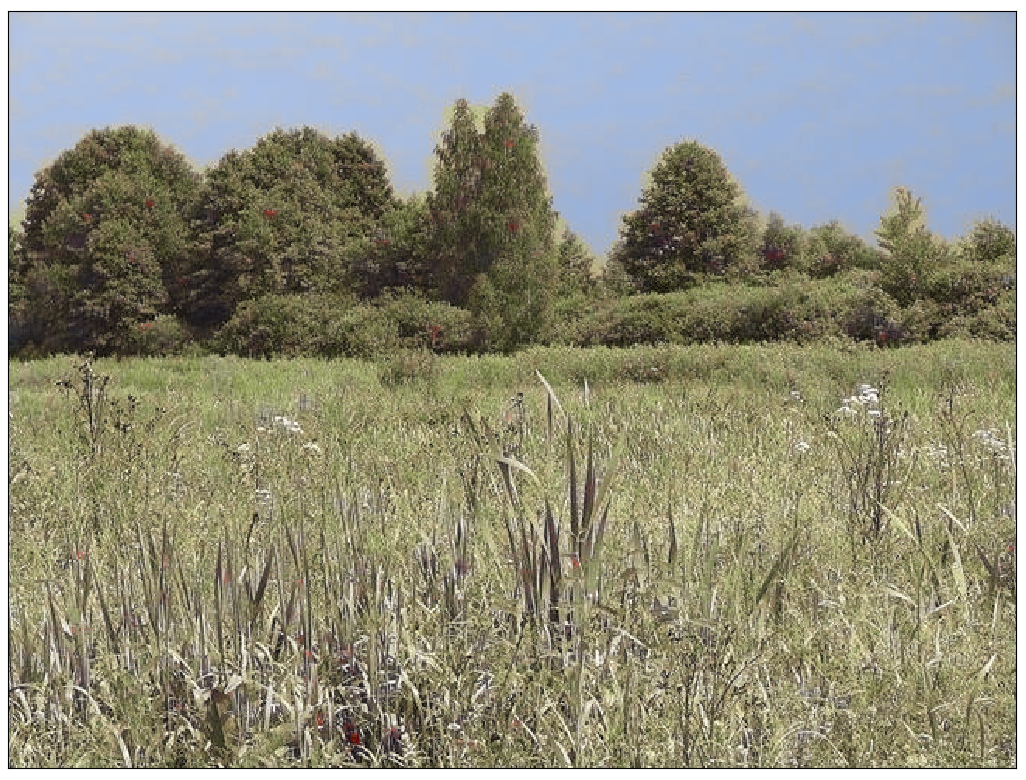
\includegraphics[width = 2in]{norm_stand}}
    \subfloat[]{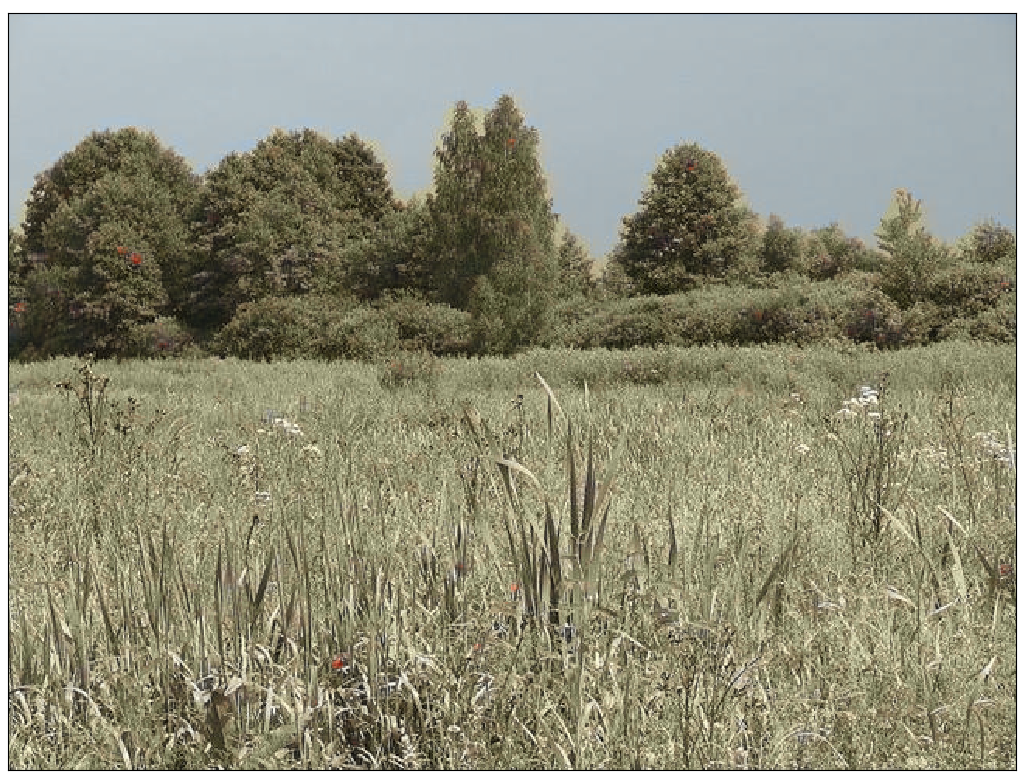
\includegraphics[width = 2in]{stand_stand}} \\
    \subfloat[]{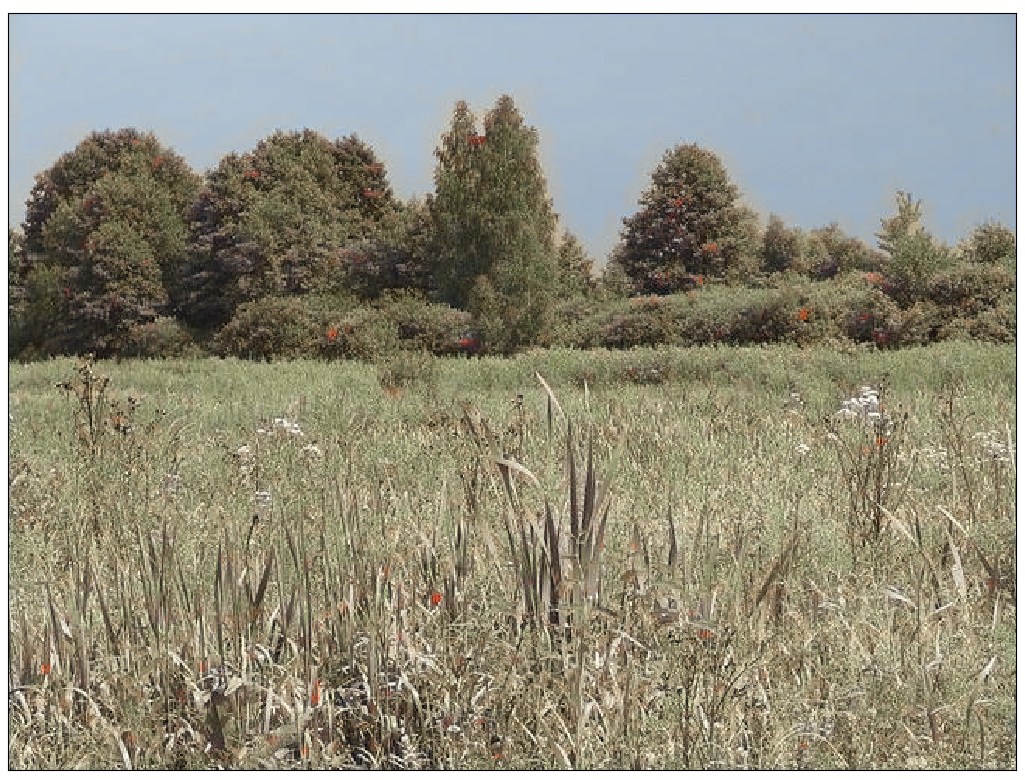
\includegraphics[width = 2in]{norm_stand_blur}}
    \subfloat[]{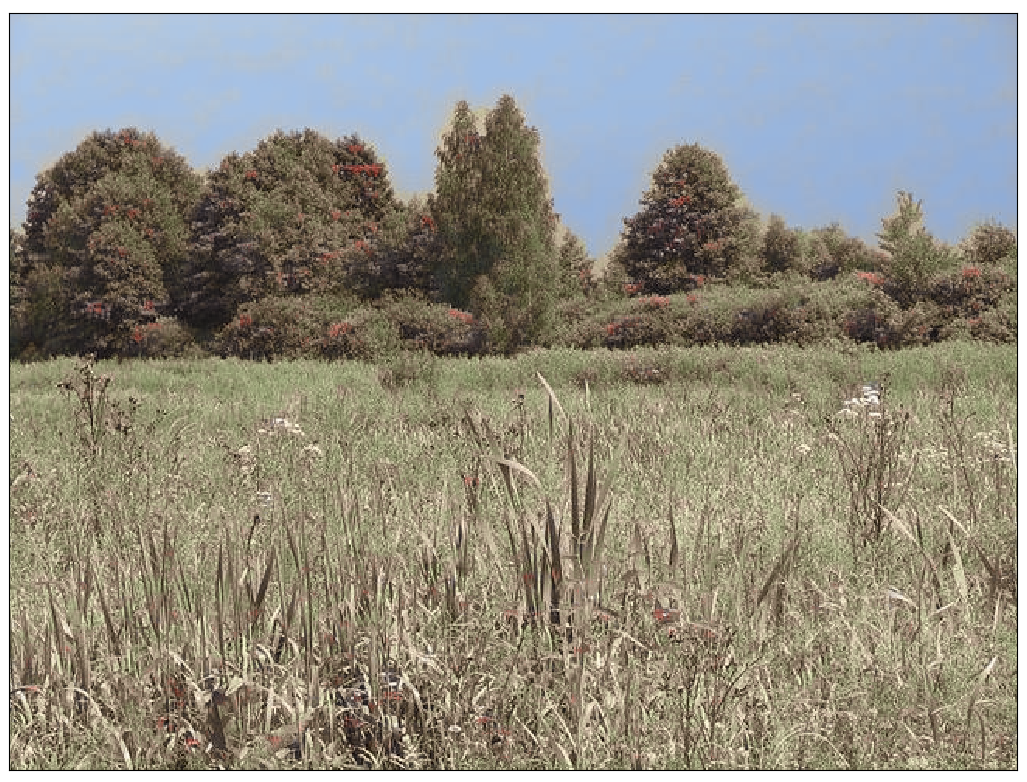
\includegraphics[width = 2in]{stand_stand_blur}} \\
    \caption[Skutki zastosowania różnych metod przetwarzania wstępnego - źródło:
    rysunek własny na podstawie
    \url{https://pl.wikipedia.org/wiki/Plik:PL_Bagno_Calowanie_2.jpg}]
    {Skutki zastosowania różnych metod przetwarzania wstępnego}
    \label{fig:porownanie_preprocessing}
  \end{figure}

  \noindent\begin{table}[H]
    \center
    \begin{tabular}{|c | c | c| }
     \hline
     Konfiguracja & Przetwarzanie danych wejściowych & Przetwarzanie danych
     referencyjnych \\ [0.5ex]
    \hline
    a & Normalizacja & Normalizacja \\ \hline
    b & Normalizacja & Standaryzacja \\ \hline
    c & Standaryzacja & Standaryzacja \\ \hline
    d & Normalizacja oraz rozmycie gaussowskie & Standaryzacja \\ \hline
    e & Standaryzacja oraz rozmycie gaussowskie & Standaryzacja \\ \hline
    \end{tabular}
    \caption{Szczegóły konfiguracji przetwarzania wstępnego.}
    \label{table:preprocessing}
  \end{table}

  \noindent
  Rezultaty przetwarzania wstępnego:
  \begin{enumerate}[label=(\alph*)]
    \item W pierwszej przetestowanej konfiguracji została zastosowana najprostsza
    metoda przetwarzania wstępnego - normalizacja, po jej zastosowaniu wartości wejścia sieci
    (składowa \textit{L}) oraz wartości referencyjne (rzeczywiste składowe
    \textit{A} i \textit{B}) były przeskalowane do przedziału od -0.5 do 0.5. Zabieg ten miał na
    celu usprawnić trening modelu z przyczyn opisanych w punkcie
    \ref{Przetwarzanie wstępne danych}. Jednakże można zauważyć, że rezultaty
    uzyskane przy tej konfiguracji prezentują się najgorzej w porównaniu z
    pozostałymi konfiguracjami, barwy na obrazie są przytłumione oraz mało
    różnorodne. Dowodzi to, że w przypadku rozważanej problematyki najprostsze
    rozwiązanie jest niewystarczające.
    \item W tym przypadku można zaobserwować znacznie lepsze rezultaty niż dla
    poprzedniej konfiguracji, Zastosowanie standaryzacji na danych referencyjnych
    znacznie usprawniło proces aktualizacji wag sieci w trakcie szukania minimum
    globalnego na płaszczyźnie funkcji celu. Generowane kolory są kontekstowo
    prawdopodobne dla kolorowanych powierzchni oraz cechują się wysokim stopniem
    nasycenia, co pozytywnie przekłada się na ich odbiór przez obserwatora. Ta
    konfiguracja została wybrana jako dająca najlepsze efekty z przedstawionych
    opcji.
    \item Kierując się sukcesem standaryzacji w konfiguracji (b) ocenione
    zostały rezultaty zastosowanie tej metody również dla danych wejściowych.
    Niestety zabieg ten nie przyniósł oczekiwanego polepszenia wyników
    modelu. Barwy na obrazie wyjściowym są mniej różnorodne oraz o
    niższej saturacji niż dla konfiguracji (b), ale za to o wyższej saturacji
    niż dla konfiguracji (a). Świadczy to, że w rozważanym zagadnieniu
    standaryzacja składowej luminacji nie wpływa pozytywnie na proces uczenia.
    Może to być spowodowane utratą kluczowych informacji o powiązaniach pomiędzy
    jasnością, a barwą, w przypadku przeskalowania składowej \textit{L}, tak aby
    uzyskać zerową wartość średnią oraz jednostkowe odchylenie standardowe.
    \item W tej konfiguracji została podjęta próba polepszenia rezultatów
    uzyskanych dla konfiguracji (b) poprzez zastosowanie dodatkowo rozmycia
    gaussowskiego na znormalizowanych danych wejściowych. Operacja ta miała na celu
    zmniejszyć wyraźność detali na obrazie, aby uwydatnić kluczowe cechy charakterystyczne
    powierzchni identyfikowanych przez warstwy konwolucyjne. Dzięki temu trenowany
    model miał się nauczyć rozpoznawać prawidłowo powierzchnie bez względu na
    przesłaniające je drobne obiekty oraz zawarte w tych powierzchniach detale
    nie zmieniające rodzaju tych powierzchni. Niepożądane by było,
    aby model inaczej nauczył się kolorować niebo w zależności czy na tle tego
    nieba występuje jakiś drobny obiekt taki jak ptak. Jednakże analizując
    Rysunek \ref{fig:porownanie_preprocessing} można dojść do wniosku, że nie
    przyniosło to oczekiwanych rezultatów, wbrew przeciwnie, obniżyło to jakość
    kolorowania względem konfiguracji bez rozmycia gaussowskiego, co wyraźnie
    widać po mniej intensywnych barwach na obrazie.
    \item Zastosowanie rozmycia gaussowskiego opisane dla konfiguracji (d)
    zostało także przetestowane w połączeniu z konfiguracją (c). W tym
    przypadku widać, że odniosło to pożądany efekt. Generowane kolory są znacznie
    bardziej nasycone niż dla konfiguracji (c) oraz pasują kontekstowo do
    powierzchni, na którą zostały nałożone. Wynika z tego, że w przypadku, kiedy zastosowanie
    standaryzacja na składowej \textit{L} może mieć niekorzystne skutki, to
    można je zredukować używają właśnie rozmycia gaussowskiego. Aczkolwiek
    porównując wyniki tej konfiguracji z wynikami konfiguracji (b) widać, że
    nie jest ona konfiguracją najbardziej odpowiednią dla rozważanego
    rozwiązania.
  \end{enumerate}

  \noindent
  Bazując na efektach wizualnych różnych konfiguracji do modelu końcowego
  została zastosowana konfiguracja (b) składająca się z operacji
  normalizacji składowej wejściowej sieci \textit{L} oraz standaryzacji
  referencyjnych składowych \textit{A} oraz \textit{B}.

  \subsubsection{Model końcowy - wnioski}

  Analizując uzyskane rezultaty dla modelu końcowego, można stanowczo
  stwierdzić, że sieci FCN zdecydowanie nadają się jako rozwiązanie problematyki kolorowania
  czarno-białych obrazów. Ich niezwykłe zdolności do adaptacji oraz wyjątkowa
  biegłość w zapamiętywaniu i identyfikowanie istotnych wzorców świetnie współgrają
  przy generowaniu prawdopodobnych barw pasujących do kolorowanych powierzchni.
  Jednakże przedstawione rozwiązanie nie jest idealne, jego dużą wadą jest
  słabo rozwinięta umiejętność do kolorowania przez modeli drobnych detali na obrazach.
  Aby zniwelować tę wadę należałoby znacząco zmodyfikować model oraz podejście do
  danej problematyki.

  Jedno z potencjalnych modyfikacji mogłoby obejmować
  wprowadzenie segmentacji obrazu oraz klasyfikacji jego segmentów w celu
  zawężenia ilości potencjalnych barw prawdopodobnych dla analizowanego segmentu obrazu.
  Model w trakcie treningu uczyłby się możliwych kolorów oddzielnie dla wszystkich
  występujących na obrazach klas zamiast dla całego obrazu jako całość,
  zmniejszyłoby to wpływ obiektów na siebie nawzajem i prawdopodobnie zwiększyło
  zdolności sieci do kolorowanie pomniejszych detali występujących na obrazach.
  Ponadto umożliwiłoby to wykorzystanie większych oraz bardziej różnorodnych
  zbiorów treningowych, co zwiększyłoby uniwersalność tego rozwiązania.
  Jednakże takie podejście wymagałoby sieci o znacznie większej architekturze,
  co przekłada się na o wiele wyższe zapotrzebowanie na moc obliczeniową często
  ciężko dostępną bez wyspecjalizowanego sprzętu.

  Pomimo niedoskonałości przedstawionego modelu końcowego należy podkreślić jego
  użyteczność w półautomatycznym kolorowaniu czarno-białych obrazów. Jak można
  było zauważyć zadowalająco radzi sobie on z kolorowaniem tła obrazów oraz
  powierzchni o mało różnorodnej kolorystyce. Można wykorzystać to do wstępnego
  pokolorowania czarno-białego obrazu, a następnie tylko innymi metodami uzupełnić
  ubytki koloru oraz poprawić barwy wymagających tego detali. Takie podejście
  jest znacznie bardziej efektywne niż przykładowo kolorowanie obrazu ręcznie od
  początku do końca.


\section{Podsumowanie}

\begin{thebibliography}{99} %{99} numery co najwyżej dwucyfrowe

  \bibitem{gan} Ian J.~Goodfellow, Jean~Pouget-Abadie, Mehdi~Mirza, Bing~Xu, David~Warde-Farley, Sherjil~Ozair, Aaron~Courville, Yoshua~Bengio:
  \emph{Generative Adversarial Networks}, arXiv ('2014)

  \bibitem{neural_photo_editor} Andrew Brock, Theodore Lim, J.M. Ritchie,
  Nick Weston:
  \emph{NEURAL PHOTO EDITING WITH INTROSPECTIVE ADVERSARIAL NETWORKS}, arXiv ('2017)

  \bibitem{cnn} Tianyi~Liu, Shuangsang~Fang, Yuehui~Zhao, Peng~Wang, Jun~Zhang:
  \emph{Implementation of Training Convolutional Neural Networks}, arXiv ('2015), s.2.

  \bibitem{deeplearn} Ian~Goodfellow, Yoshua~Bengio, Aaron~Courville:
  \emph{Deep Learning}, ('2016), s.342., s.82.

  \bibitem{colorful_image_colorization} Richard Zhang, Phillip Isola, Alexei A. Efros:
  \emph{Colorful Image Colorization}, arXiv ('2016)

  \bibitem{image_style_transfer} Leon A. Gatys, Alexander S. Ecker, Matthias Bethge:
  \emph{Image Style Transfer Using Convolutional Neural Networks}, IEEE ('2016)

  \bibitem{vgg_network} Karen Simonyan, Andrew Zisserman:
  \emph{Very Deep Convolutional Networks For Large-Scale Image Recognition}, ('2016)

  \bibitem{gan_editing} Guim Perarnau, Joost van de Weijer, Bogdan Raducanu, Jose M. Álvarez:
  \emph{Invertible Conditional GANs for image editing}, arXiv ('2016)

  \bibitem{vae} Diederik P. Kingma, Max Welling:
  \emph{Auto-Encoding Variational Bayes}, arXiv ('2014)

  \bibitem{BatchNorm} Sergey Ioffe, Christian Szegedy:
  \emph{Batch Normalization: Accelerating Deep Network Training by Reducing
  Internal Covariate Shift}, arXiv ('2015)


  \bibitem{exploding_vanishing_grad} Y. Bengio, P. Simard, P. Frasconi:
  \emph{Learning long-term dependencies with gradient descent is difficult},
  IEEE ('1994)

  \bibitem{dropout} Nitish Srivastava, Geoffrey Hinton, Alex Krizhevsky,
  Ilya Sutskever, Ruslan Salakhutdinov:
  \emph{Dropout: A Simple Way to Prevent Neural Networks from Overfitting},
  Journal of Machine Learning Research ('2014)

  \bibitem{cifar-10} A. Krizhevsky:
  \emph{Learning Multiple Layers of Features from Tiny Images},
  Master’s thesis, Department of Computer Science, University of Toronto ('2009)

  \bibitem{SmoothL1Loss} R. Girshick:
  \emph{Fast R-CNN},
  arXiv ('2015)

  \bibitem{evaluatiuon_of_relu} B. Xu, N. Wang, T. Chen, M. Li:
  \emph{Empirical Evaluation of Rectied Activations in Convolution Network},
   arXiv ('2015)

   \bibitem{pytorch} Adam Paszke, Sam Gross, Soumith Chintala, Gregory Chanan,
   Edward Yang, Zachary DeVito, Zeming Lin, Alban Desmaison, Luca Antiga, Adam Lerer:
   \emph{Automatic differentiation in PyTorch}, 31st Conference on Neural Information
   Processing Systems (NIPS 2017), Long Beach, CA, USA

  \bibitem{neuralsmithing}  Russell Reed,  Robert J MarksII:
  \emph{Neural Smithing: Supervised Learning in Feedforward Artificial Neural Networks},
  Paperback – February 17, 1999, s.155.

  \bibitem{systematic_introduction} Raul Rojas:
  \emph{Neural Networks - A Systematic Introduction},
  Springer-Verlag, Berlin, New-York, 1996, s.161.


\end{thebibliography}


\section*{Załączniki}
\addcontentsline{toc}{section}{Załączniki}  % Dodanie to TOC
  \tab Załączniki i dodatki\:



\end{document}
